\iffalse
NOTES TO SELF:
physics motivation
data sets before event selection
PID
exclusive cuts
results to show
1 slide of what needs to go from here to cross section
\fi

\section{Generator and Simulations}
    Simulations were processed to better understand the results of the exclusive data analysis. GEMC was used to process generated events through the CLAS12 fall 2018 RG-A configuration. Specifically, a generator based off the GK model and CLAS6 data - aao\_norad\footnote{https://github.com/drewkenjo/aao\_norad} - was used to generate 4 million DV$\pi^0$P events and ran through GEMC with the fall 2018 inbending configuration. Following the standard decoding and reconstruction code flow, the resultant .hipo files were then ready\footnote{/volatile/clas12/kenjo/cache/} to be analyzed the same way that the data was.
    
    The results from the simulation are compared to the results from processing the 174 runs of 2018 Fall inbending data\footnote{/cache/clas12/rg-a/production/recon/fall2018/torus-1/pass1/v0/dst/train/skim8/} through the same analysis scripts. For the sake of comparison, the vertical scale of the simulated results is scaled by the ratio of the total number of observed exclusive events from data to those from the simulation. Further note that we do not expect a good match between data and simulation before exclusivity cuts, because this simulation contained no background. Finally, this study only considers events wherein the proton was detected in the forward detector; the central detector is excluded entirely at this point in time. \\
    
    Overall, the simulation and data show a good level of agreement both in terms of kinematics and exclusivity. As the agreement is reasonable, effort can proceed to undergo acceptance and other studies to work towards an absolute cross section determination.

\section{Comparison to Data: Basic Kinematics}
    Here we show some example plots of basic particle kinematics. The polar and azimuthal angle distributions of the protons and electrons agreed well. 
    
        \begin{figure}
            \centering
            \begin{subfigure}{.45\textwidth}
                \centering
                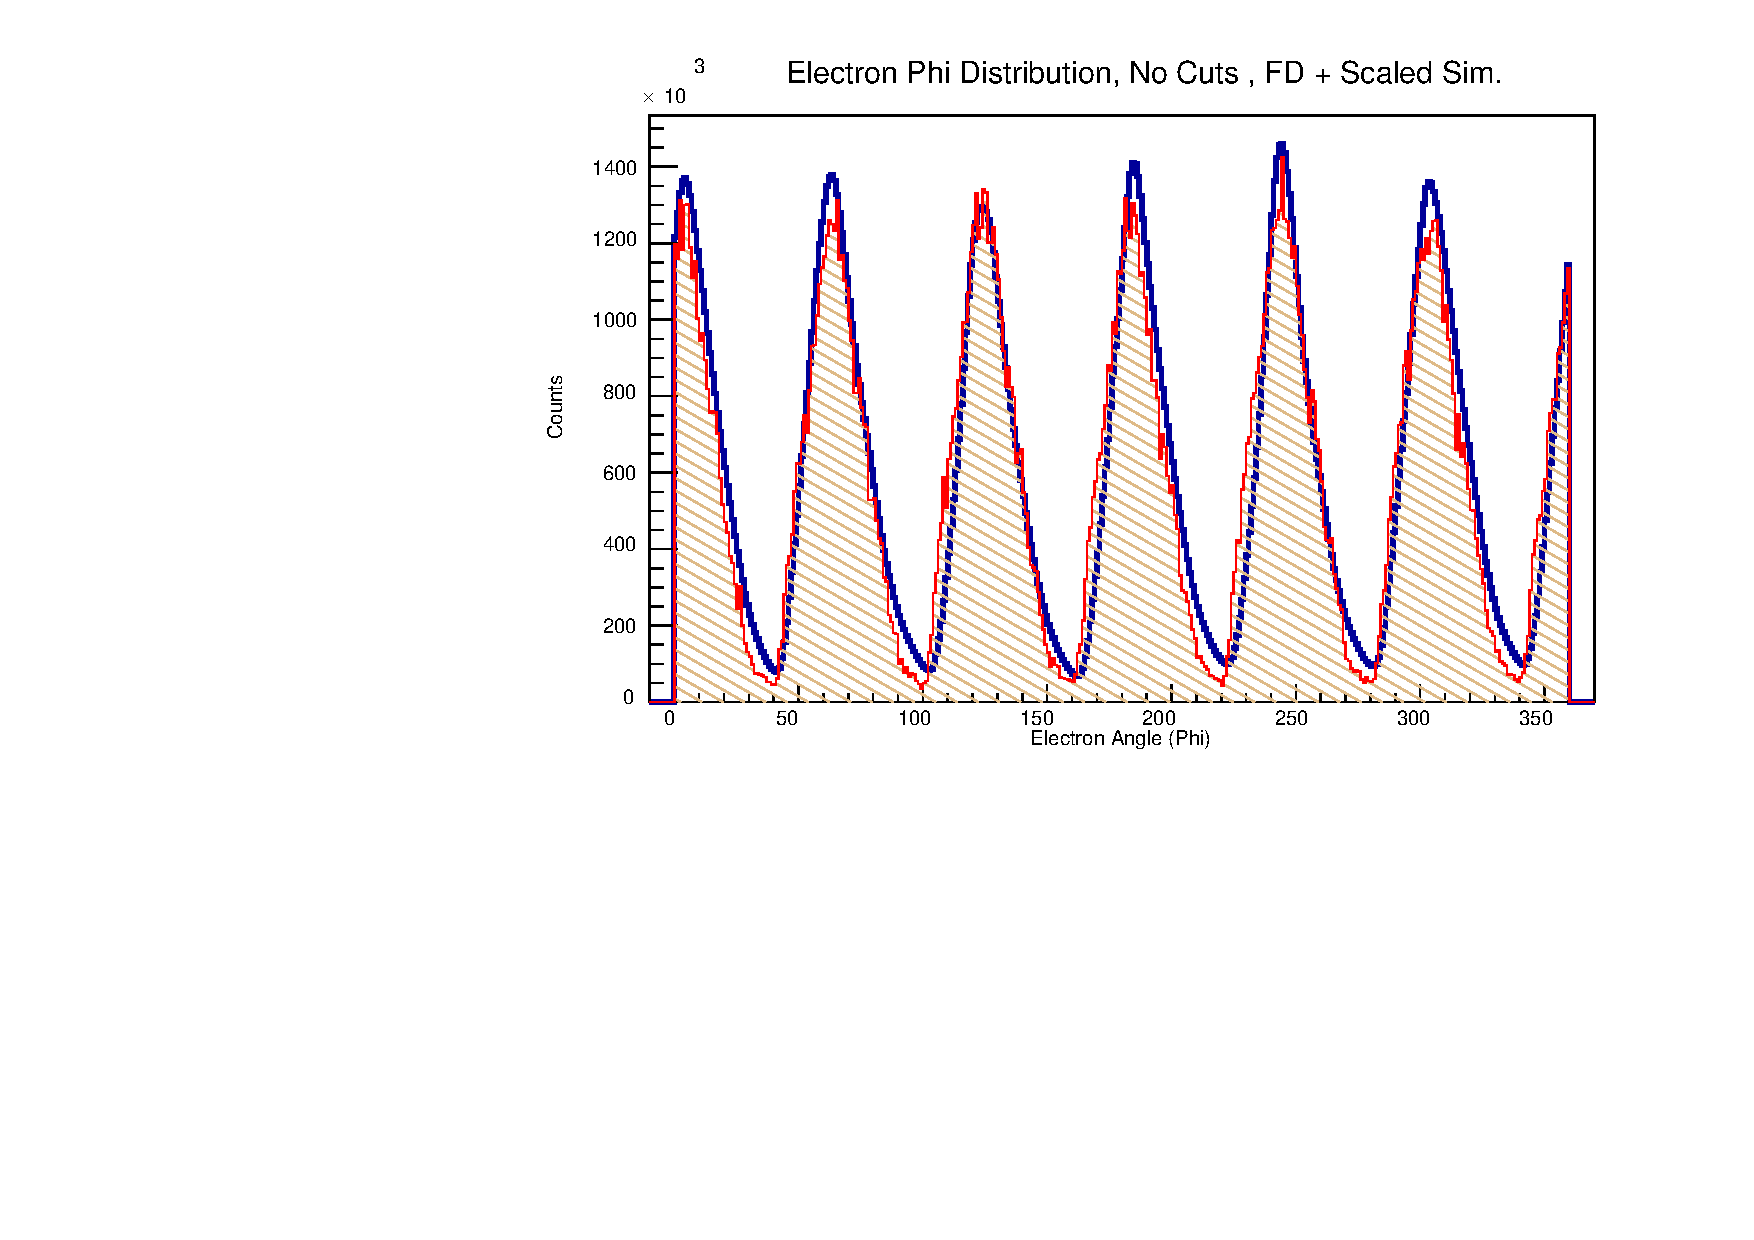
\includegraphics[width=1\textwidth]{figures/Simulation/kinematics_basic/hist_electron_phi_nocut_fd_Double.pdf}
            \end{subfigure}%
            \begin{subfigure}{.45\textwidth}
                \centering
                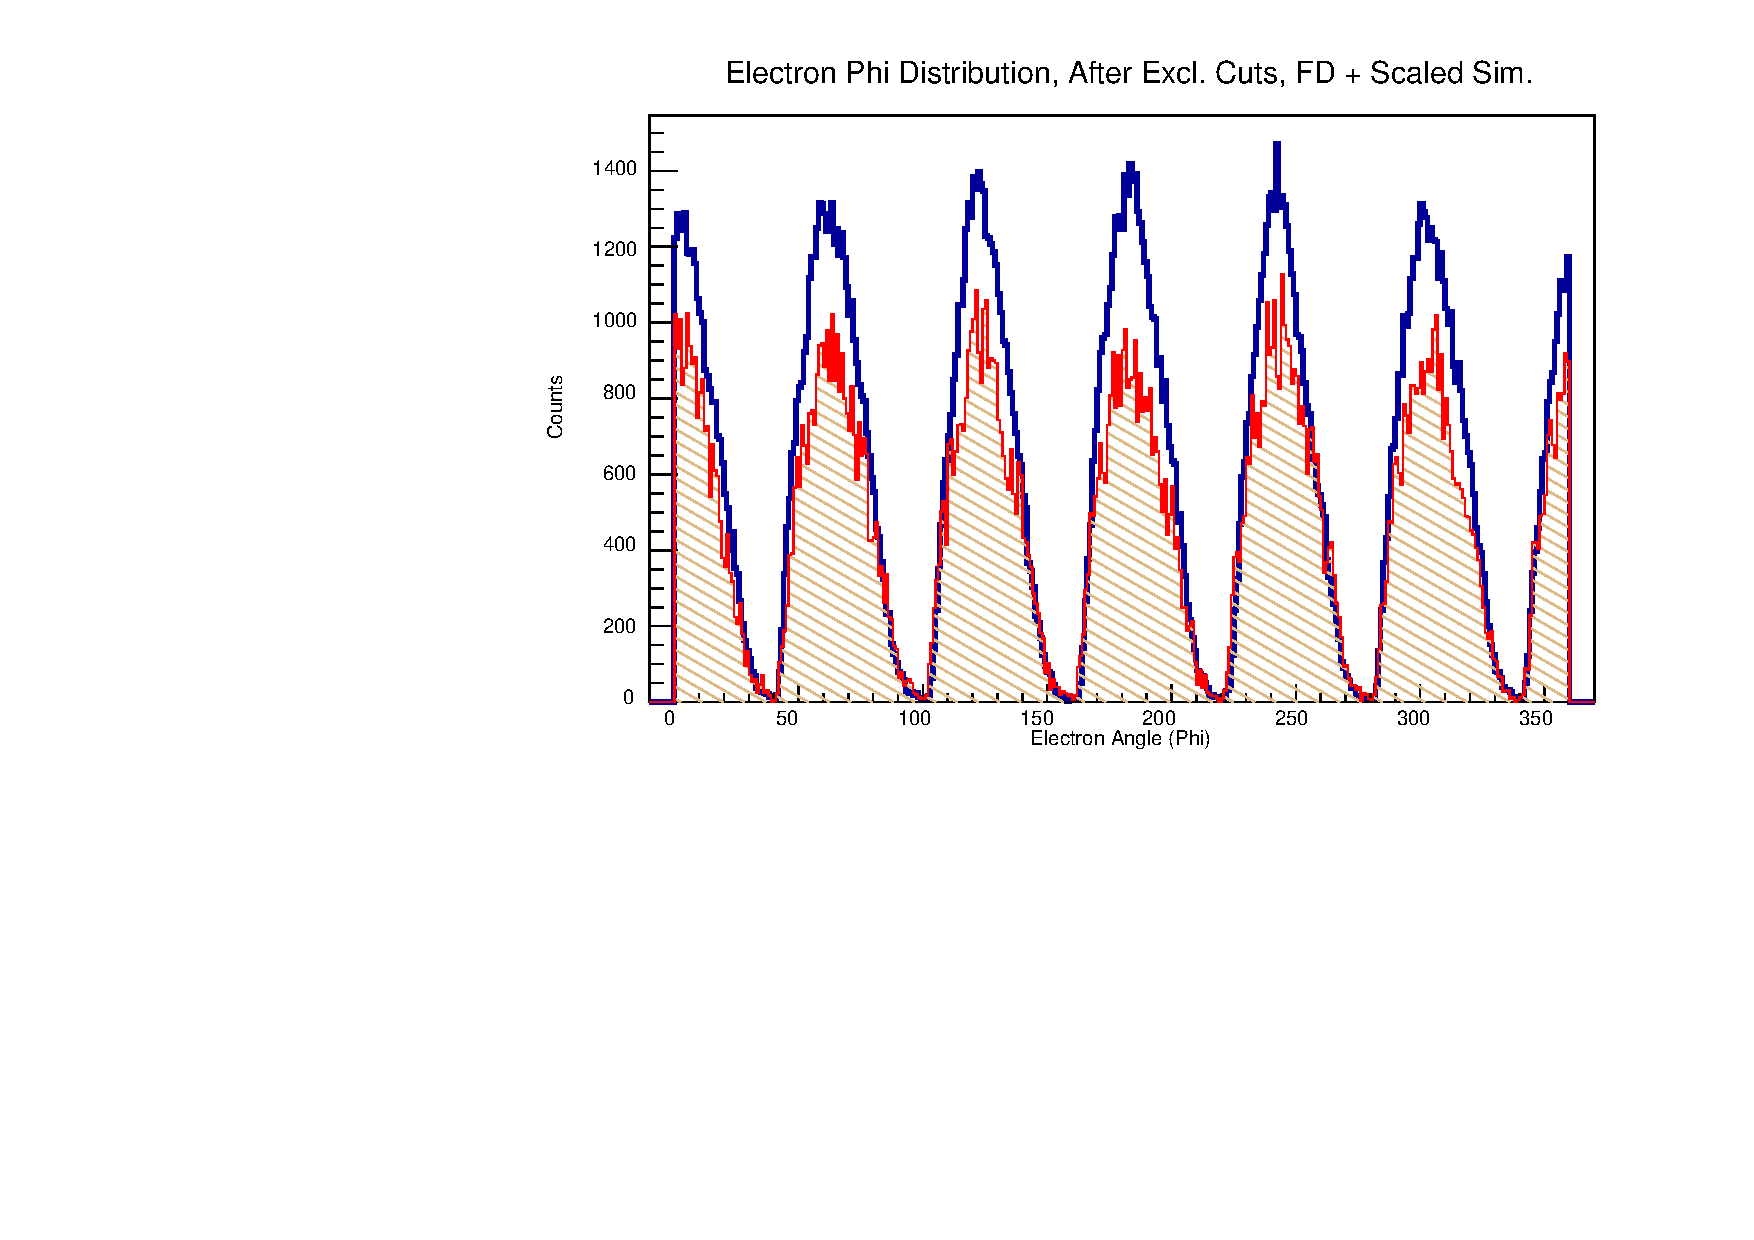
\includegraphics[width=1\textwidth]{figures/Simulation/kinematics_basic/hist_electron_phi_excut_fd_Double.pdf}
            \end{subfigure}
            \begin{subfigure}{.45\textwidth}
                \centering
                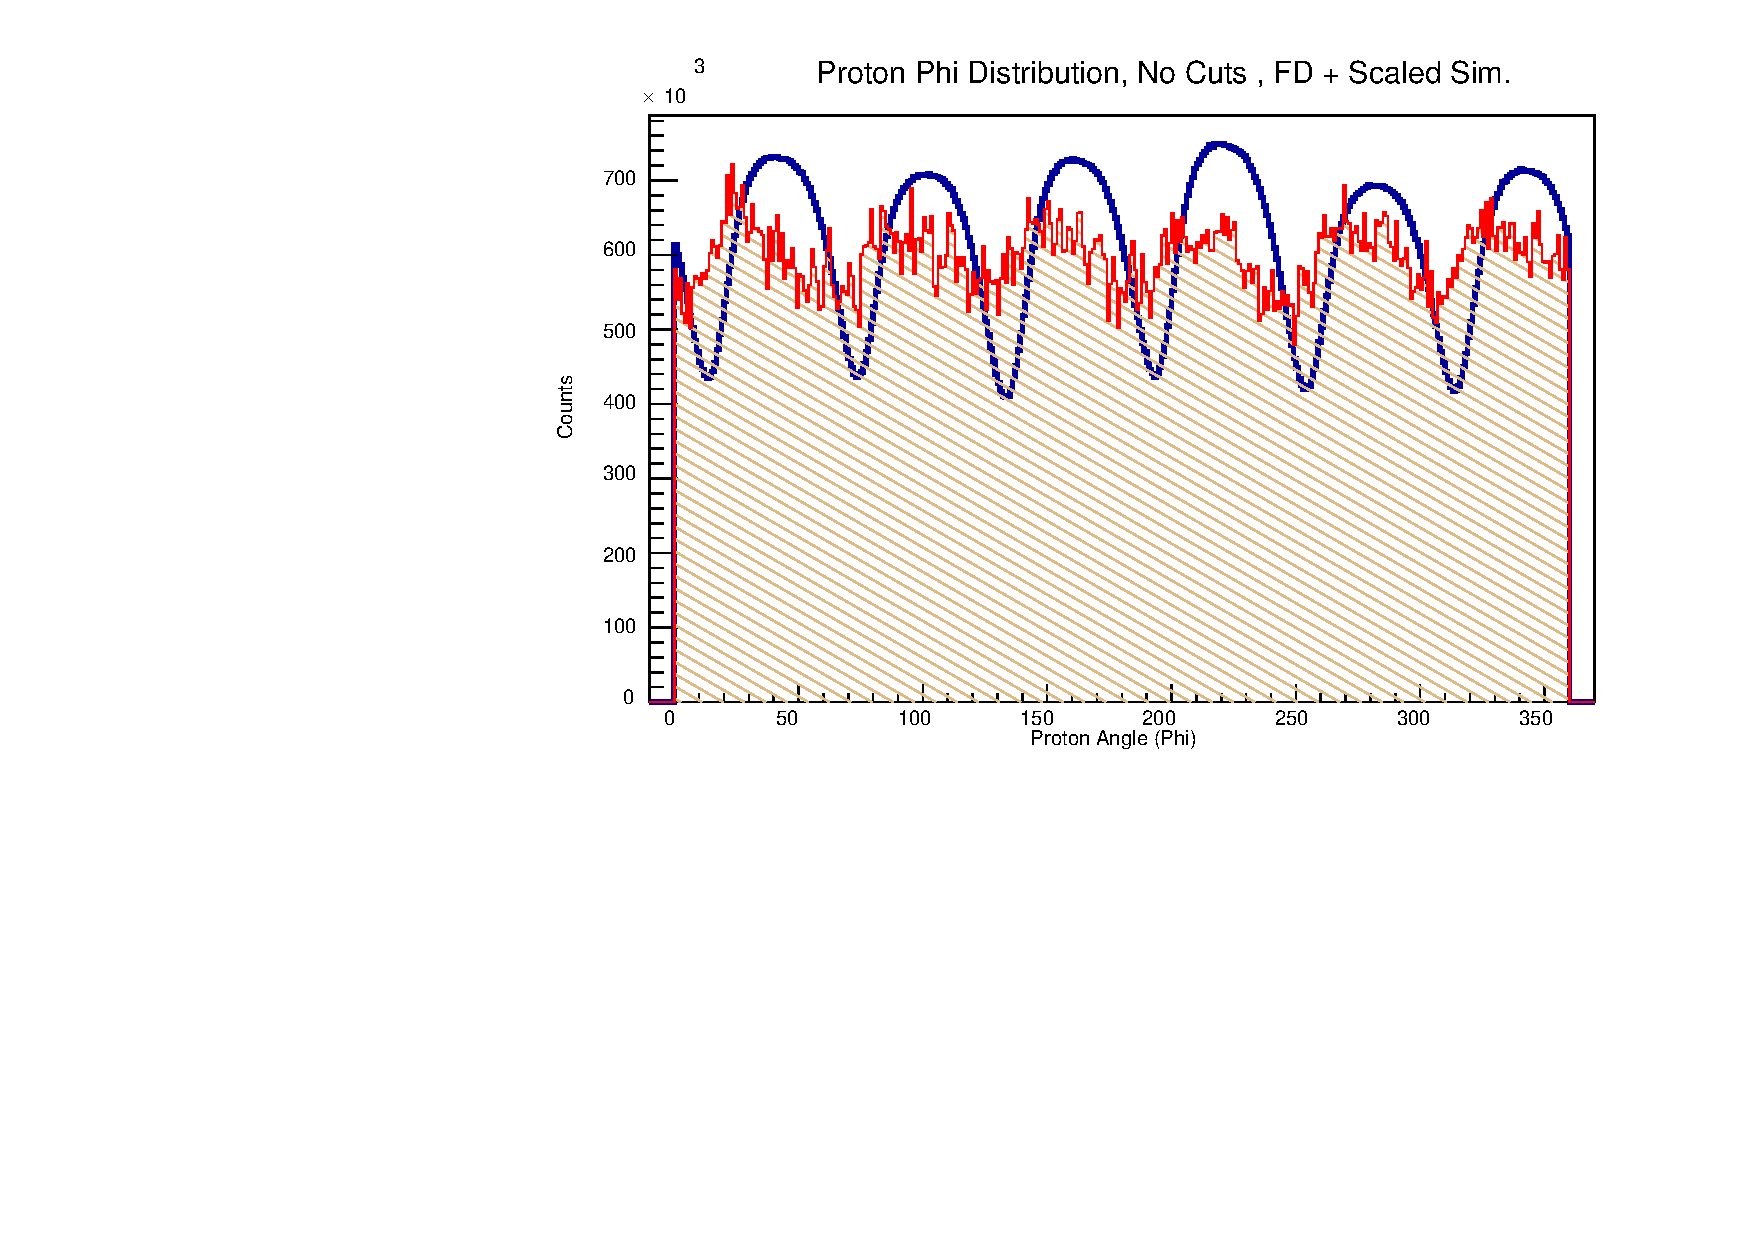
\includegraphics[width=1\textwidth]{figures/Simulation/kinematics_basic/hist_proton_phi_nocut_fd_Double.pdf}
            \end{subfigure}%
            \begin{subfigure}{.45\textwidth}
                \centering
                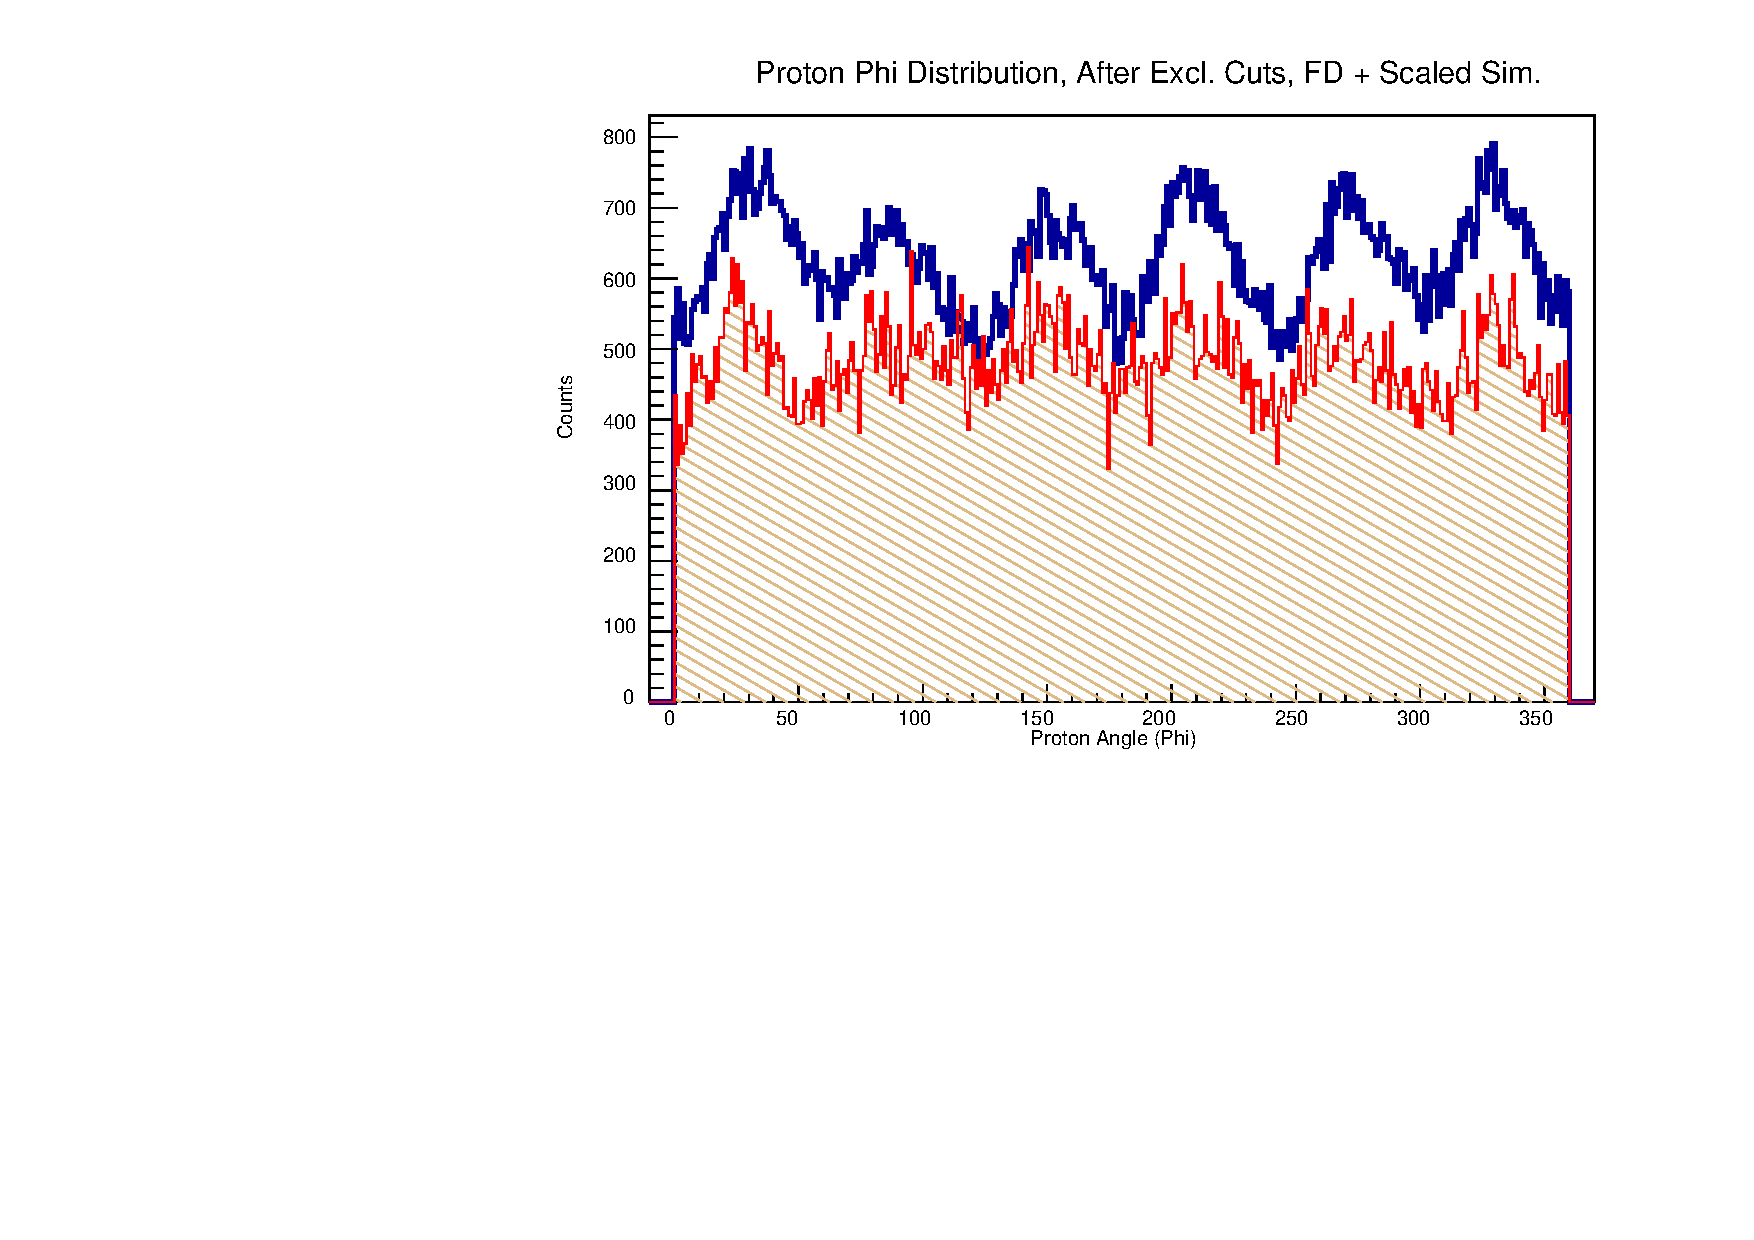
\includegraphics[width=1\textwidth]{figures/Simulation/kinematics_basic/hist_proton_phi_excut_fd_Double.pdf}
            \end{subfigure}
            \caption[short]{Electron (top) and proton (bottom) phi distributions, before exclusivity cuts (left) and after (right) for data (blue) and simulation (red)}
        \end{figure}
        
        \begin{figure}
            \centering
            \begin{subfigure}{.45\textwidth}
                \centering
                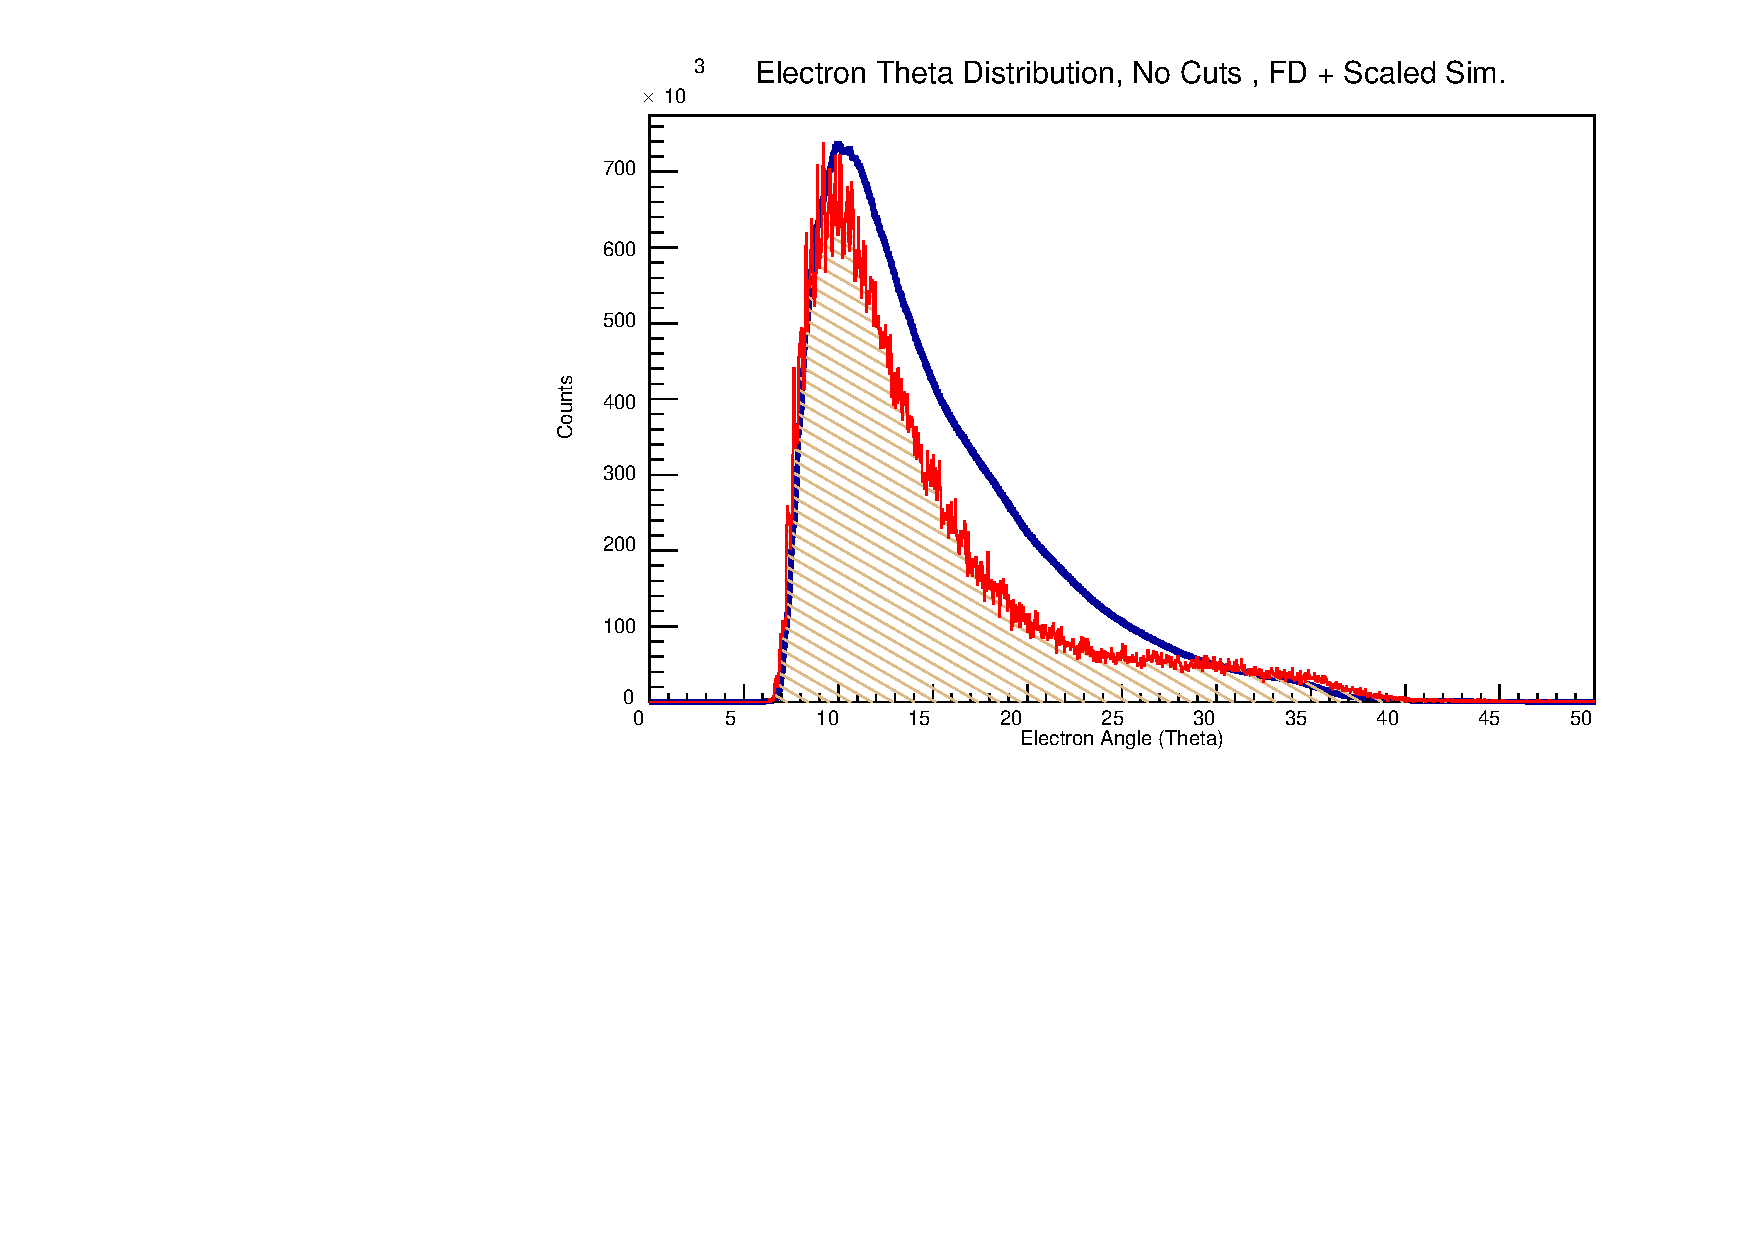
\includegraphics[width=1\textwidth]{figures/Simulation/kinematics_basic/hist_electron_theta_nocut_fd_Double.pdf}
            \end{subfigure}%
            \begin{subfigure}{.45\textwidth}
                \centering
                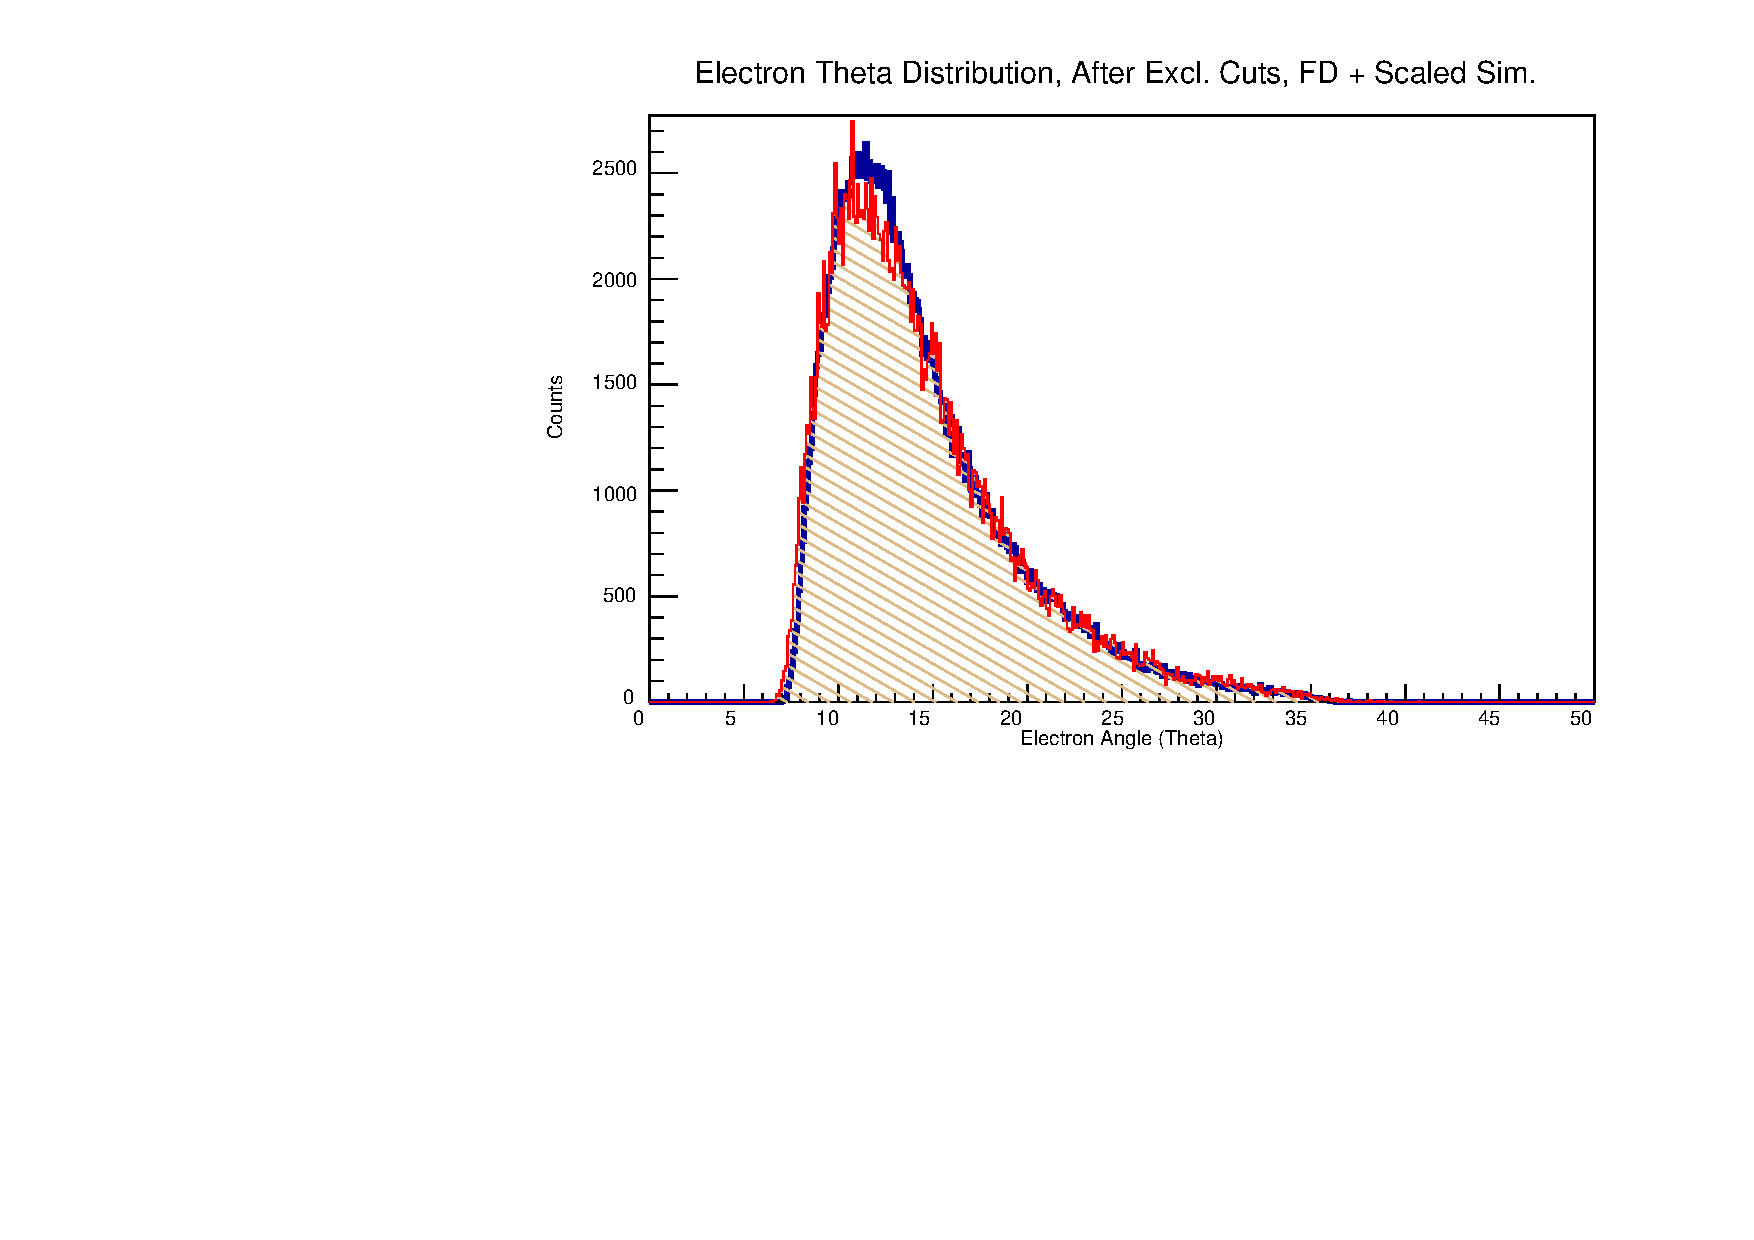
\includegraphics[width=1\textwidth]{figures/Simulation/kinematics_basic/hist_electron_theta_excut_fd_Double.pdf}
            \end{subfigure}
            \begin{subfigure}{.45\textwidth}
                \centering
                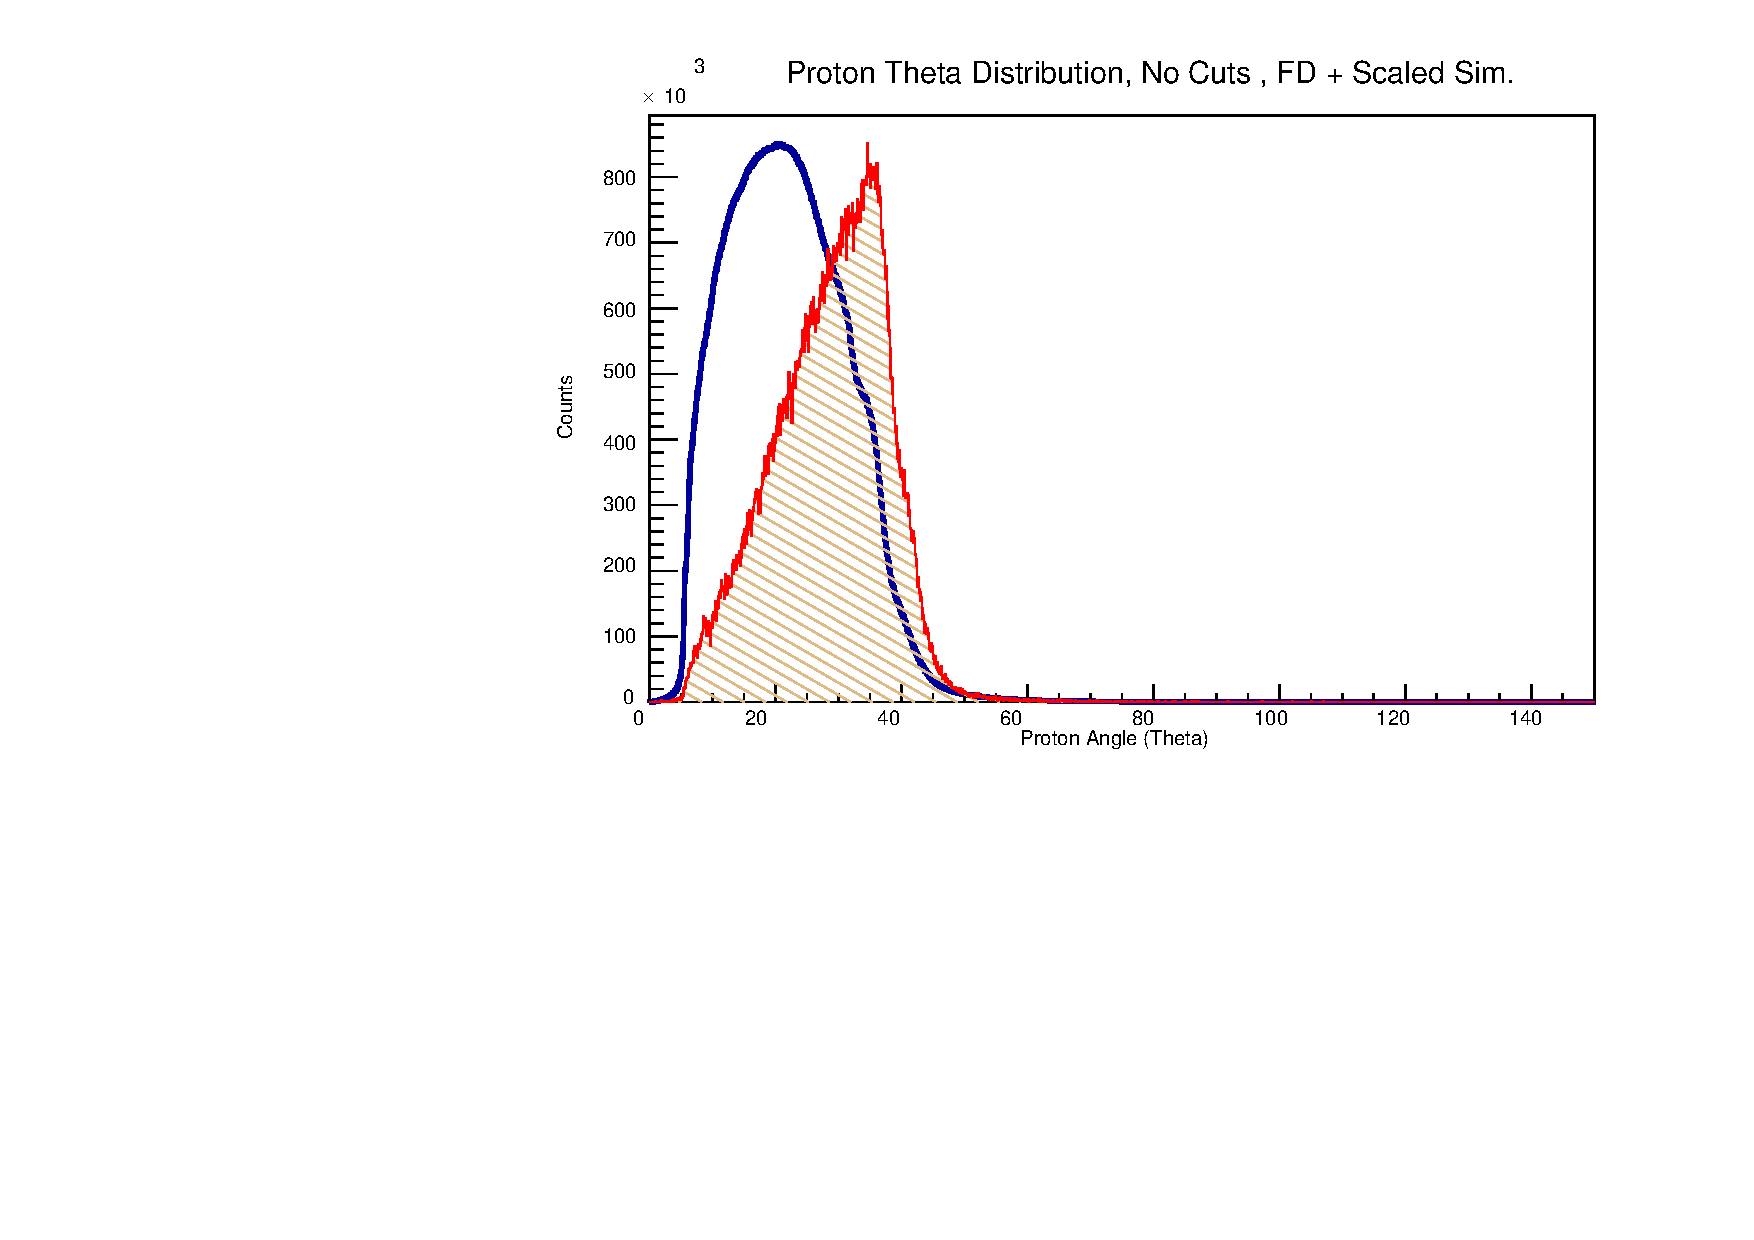
\includegraphics[width=1\textwidth]{figures/Simulation/kinematics_basic/hist_proton_theta_nocut_fd_Double.pdf}
            \end{subfigure}%
            \begin{subfigure}{.45\textwidth}
                \centering
                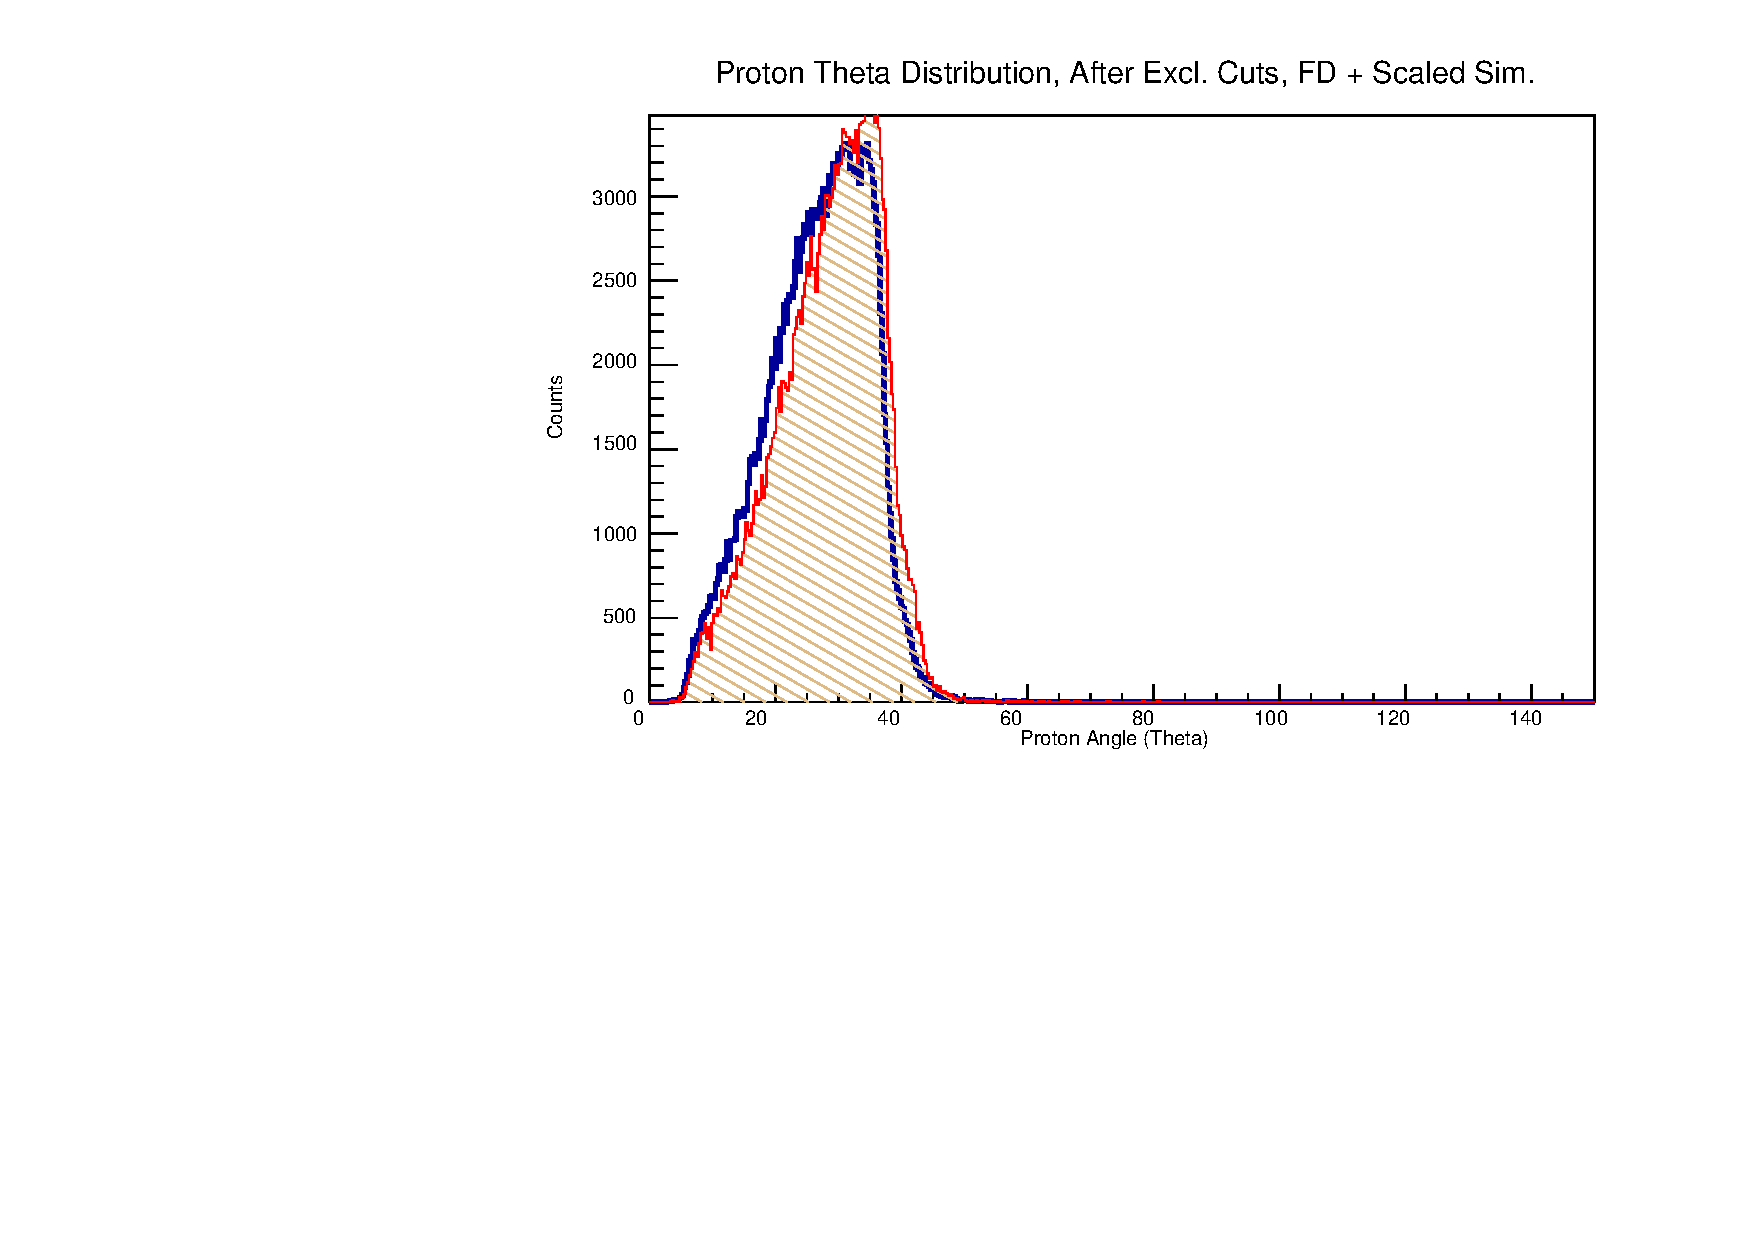
\includegraphics[width=1\textwidth]{figures/Simulation/kinematics_basic/hist_proton_theta_excut_fd_Double.pdf}
            \end{subfigure}
            \caption[short]{Electron (top) and proton (bottom) theta distributions, before exclusivity cuts (left) and after (right) for data (blue) and simulation (red)}
        \end{figure} 

    \clearpage

\section{Comparison to Data: Kinematics - Scattering Variables}
    The distributions of kinematic variables $x_B$, $Q^2$, W, and t all again showed reasonable agreement between data and simulations. Notably, here we can see that the distributions from the simulations vary considerably from the data before any exclusivity cuts, but as mentioned previously this is expected as the simulation has no background. There is good agreement after exclusivity cuts. 
    
    \subsection{Bjorken X and $Q^2$ Distributions}

        \begin{figure}[!htb]
            \centering
            \begin{subfigure}{.45\textwidth}
                \centering
                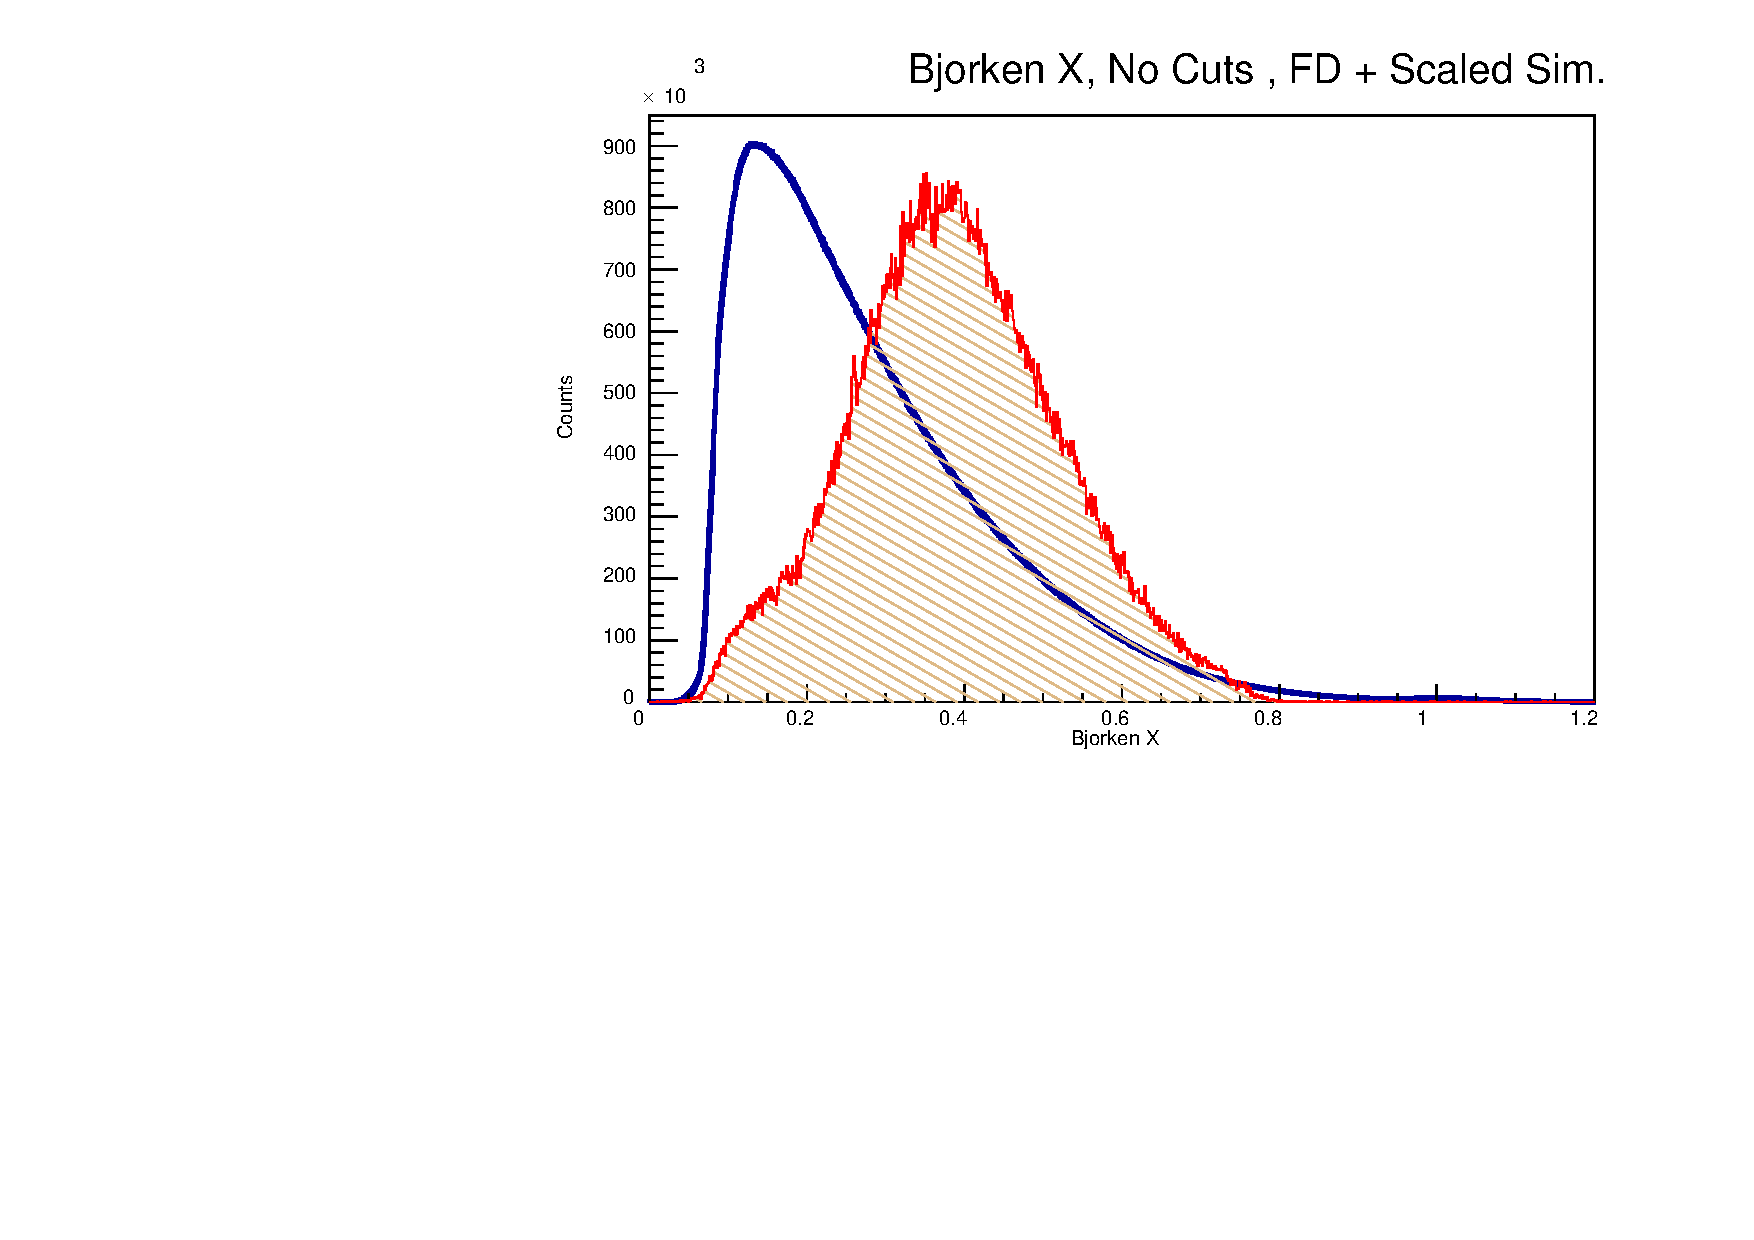
\includegraphics[width=1\textwidth]{figures/Simulation/kinematics_advanced/hist_xb_nocut_fd_Double.pdf}
            \end{subfigure}%
            \begin{subfigure}{.45\textwidth}
                \centering
                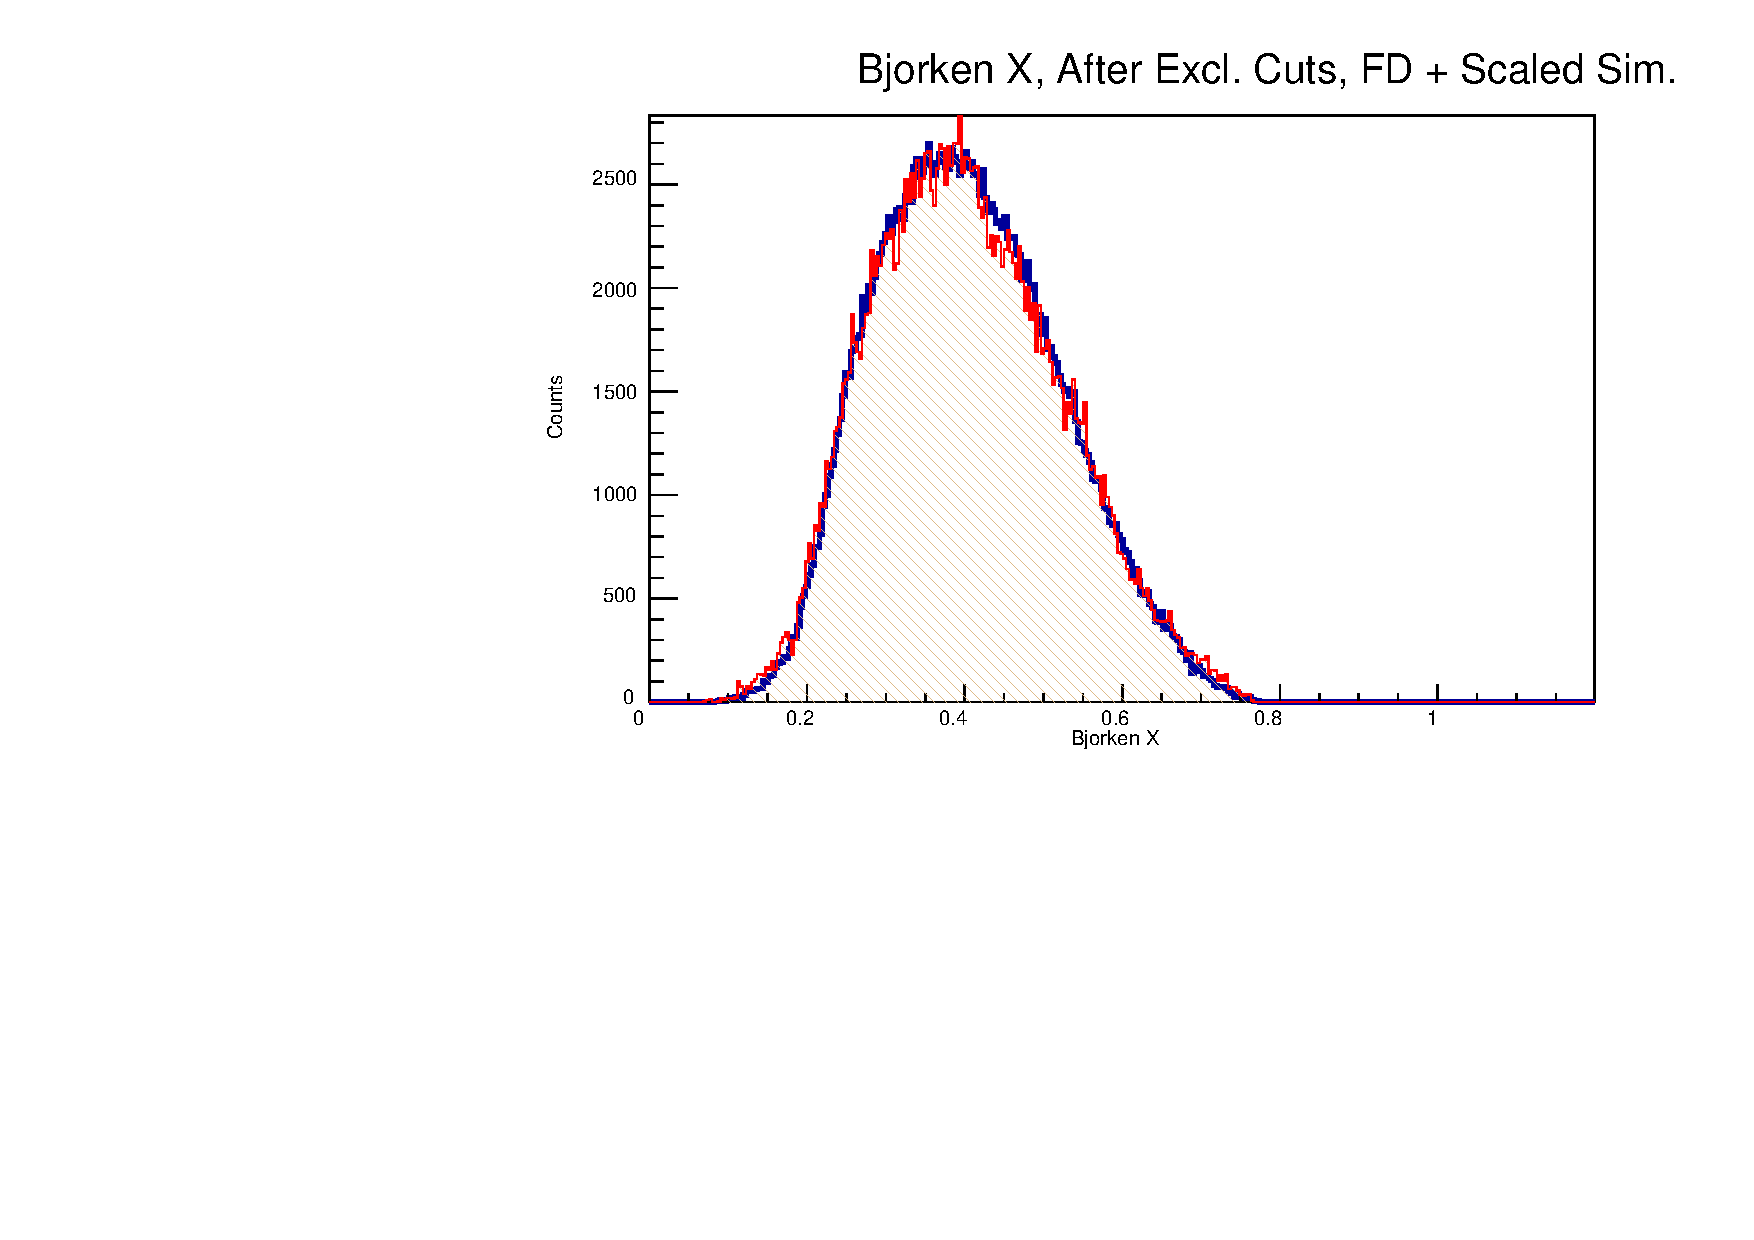
\includegraphics[width=1\textwidth]{figures/Simulation/kinematics_advanced/hist_xb_excut_fd_Double.pdf}
            \end{subfigure}
            \begin{subfigure}{.45\textwidth}
                \centering
                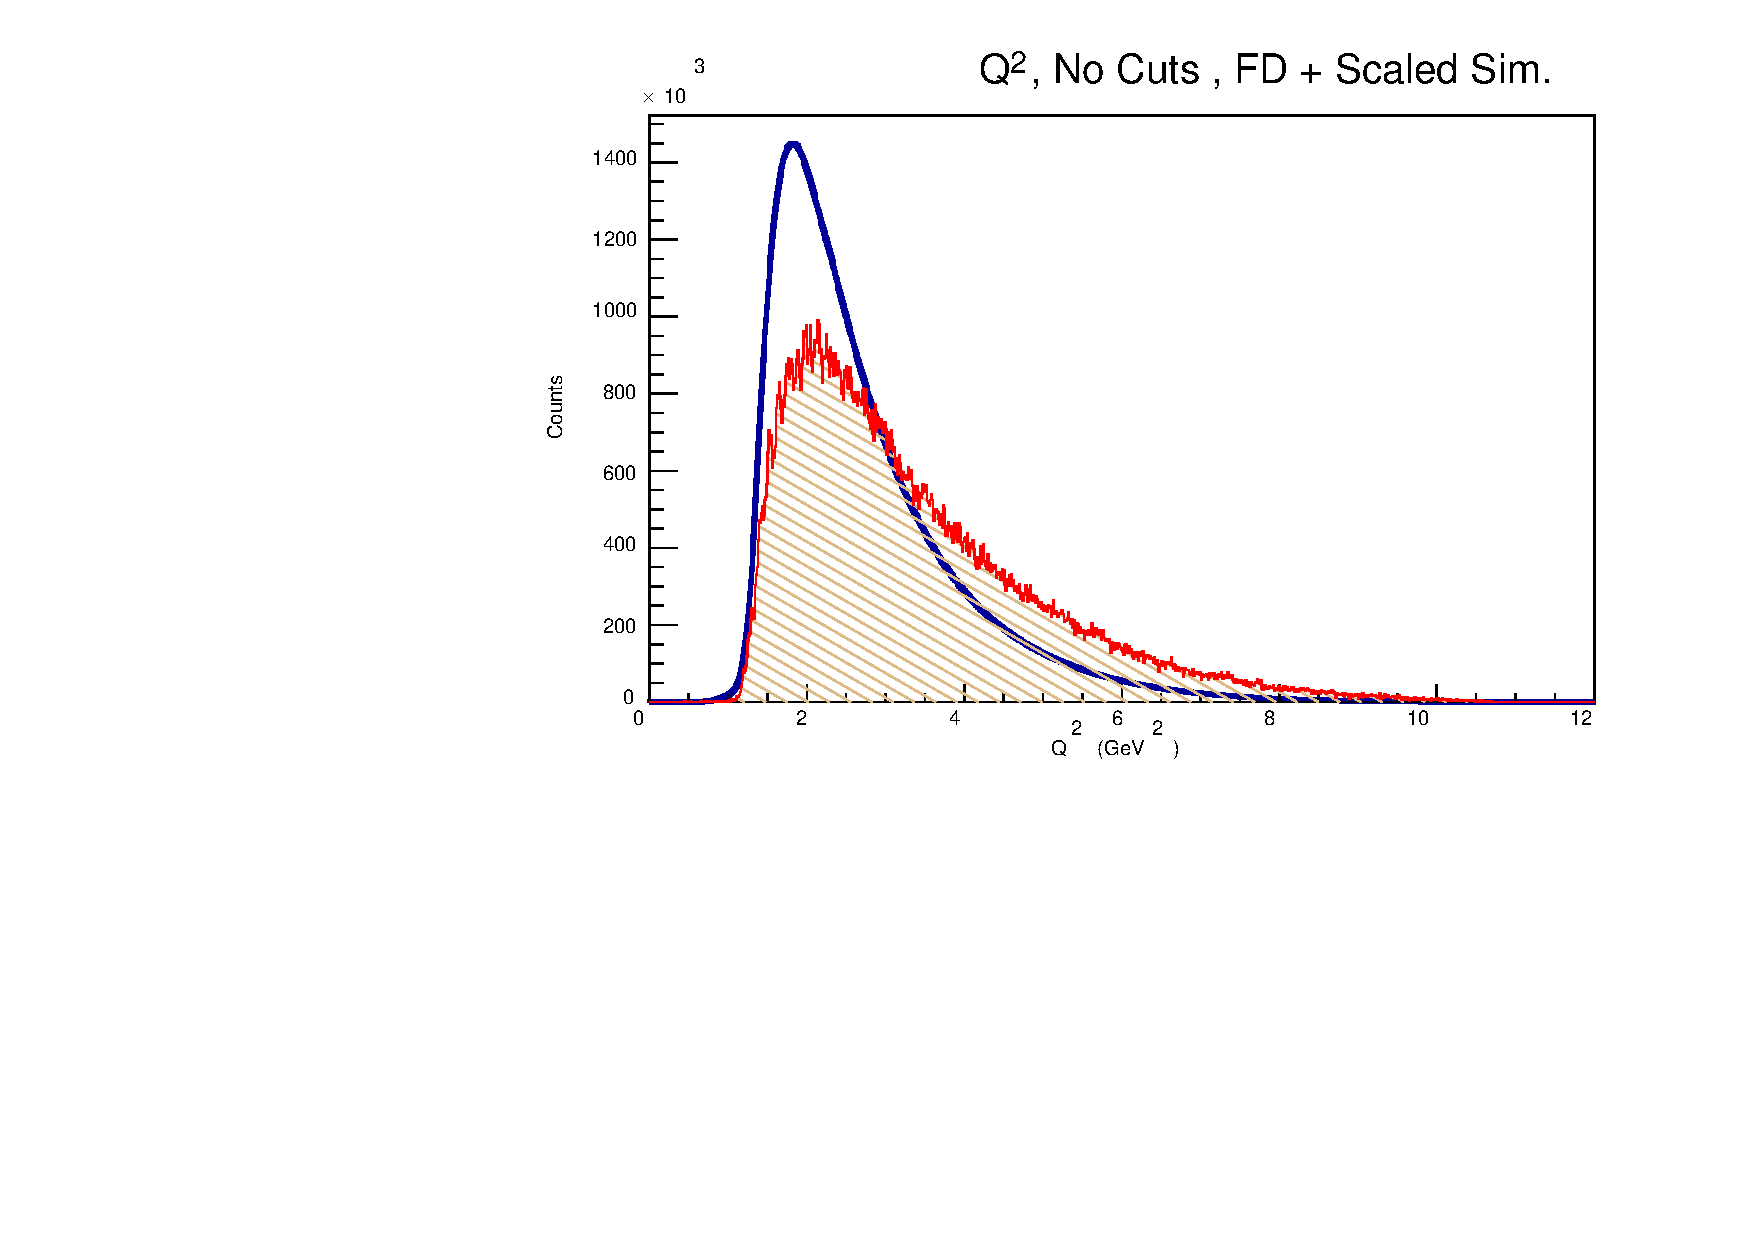
\includegraphics[width=1\textwidth]{figures/Simulation/kinematics_advanced/hist_q2_nocut_fd_Double.pdf}
            \end{subfigure}%
            \begin{subfigure}{.45\textwidth}
                \centering
                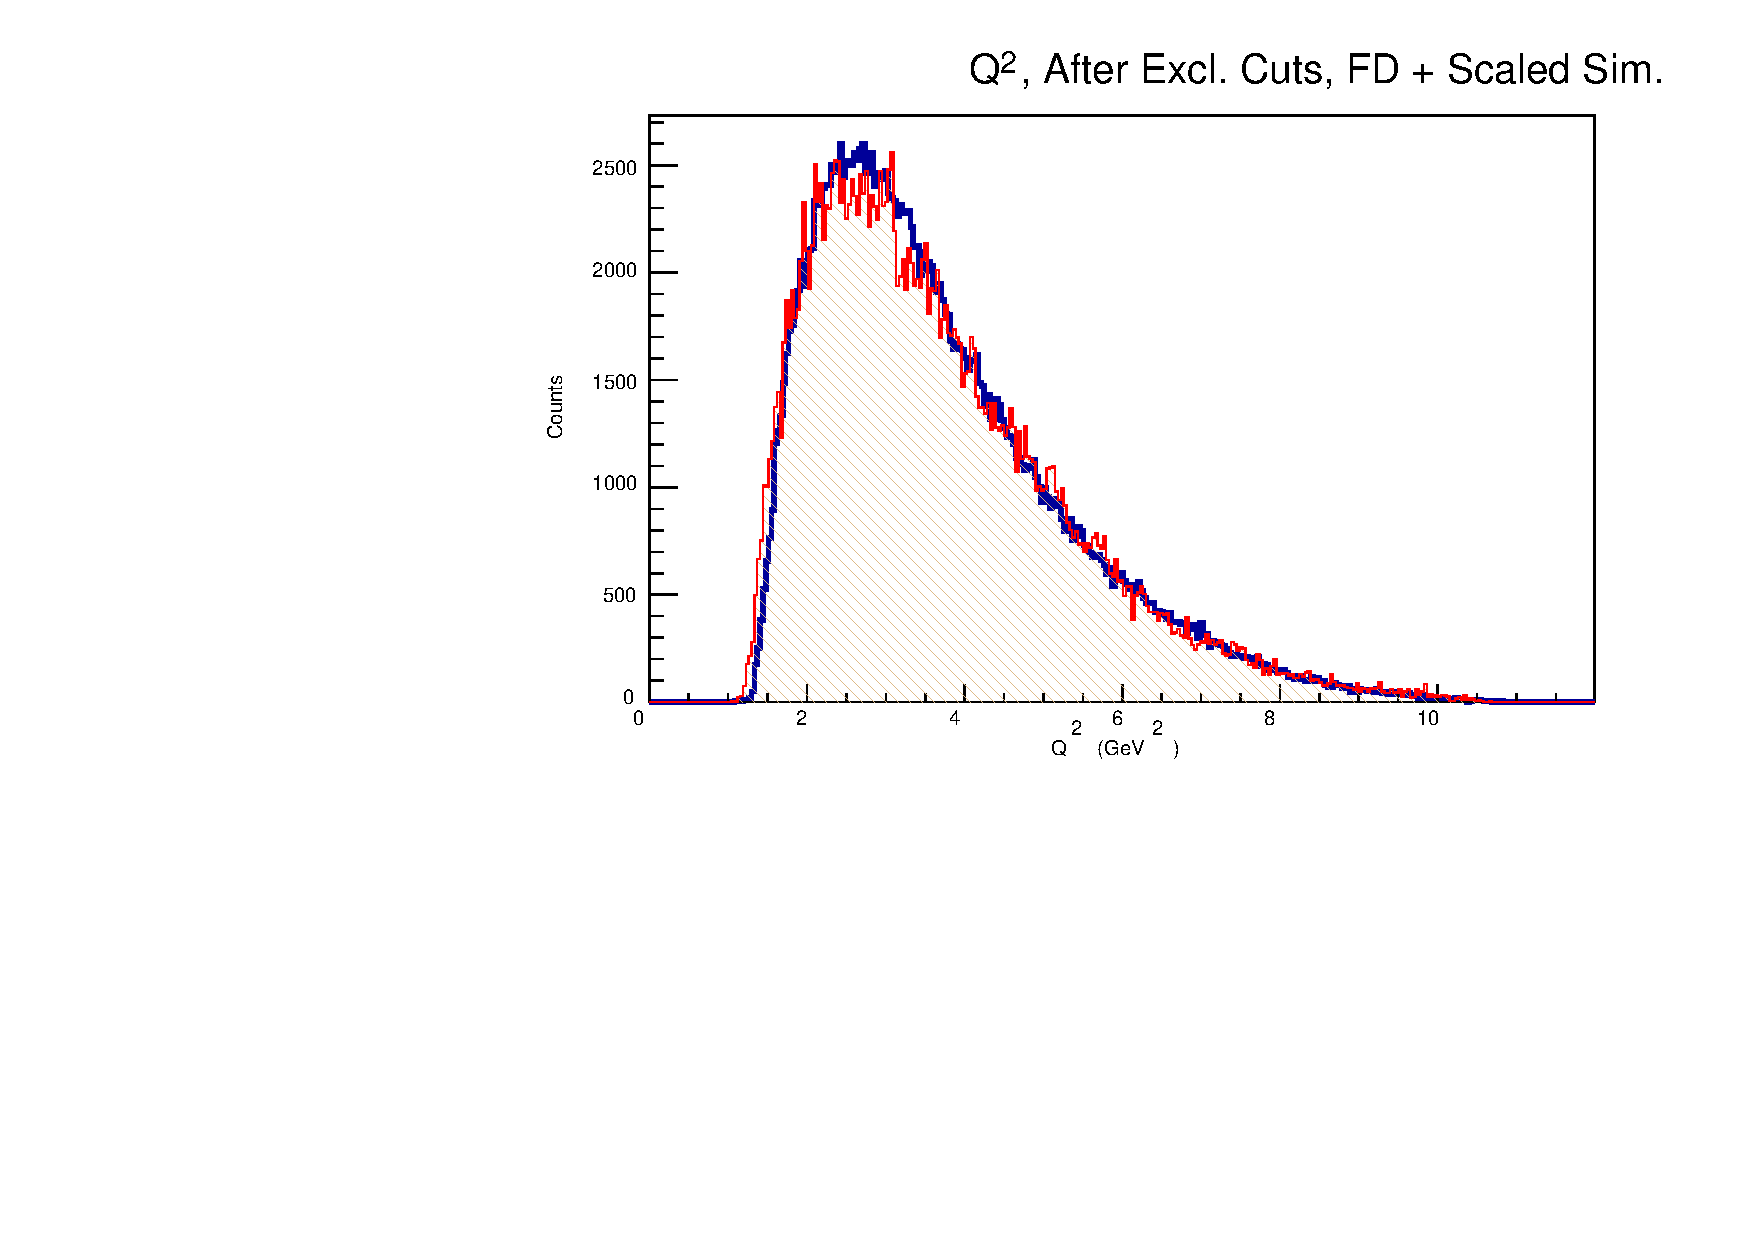
\includegraphics[width=1\textwidth]{figures/Simulation/kinematics_advanced/hist_q2_excut_fd_Double.pdf}
            \end{subfigure}
            \caption[short]{$x_B$ (top) and $Q^2$ (bottom) distributions, before exclusivity cuts (left) and after (right) for data (blue) and simulation (red)}
        \end{figure}
        
    \clearpage    
    \subsection{W and t Distributions}
    The outgoing 4-momenta W and the squared momentum transferred to the proton t similarly show reasonable overlap after exclusivity cuts are made. The W distribution before exclusivity cuts appears to be very different between data and simulation, but this is just because the simulated results had to be scaled up by a large factor to be visible in comparison with the real data, which has a significant amount of background before cuts.

        \begin{figure}[!htb]
            \centering
            \begin{subfigure}{.5\textwidth}
                \centering
                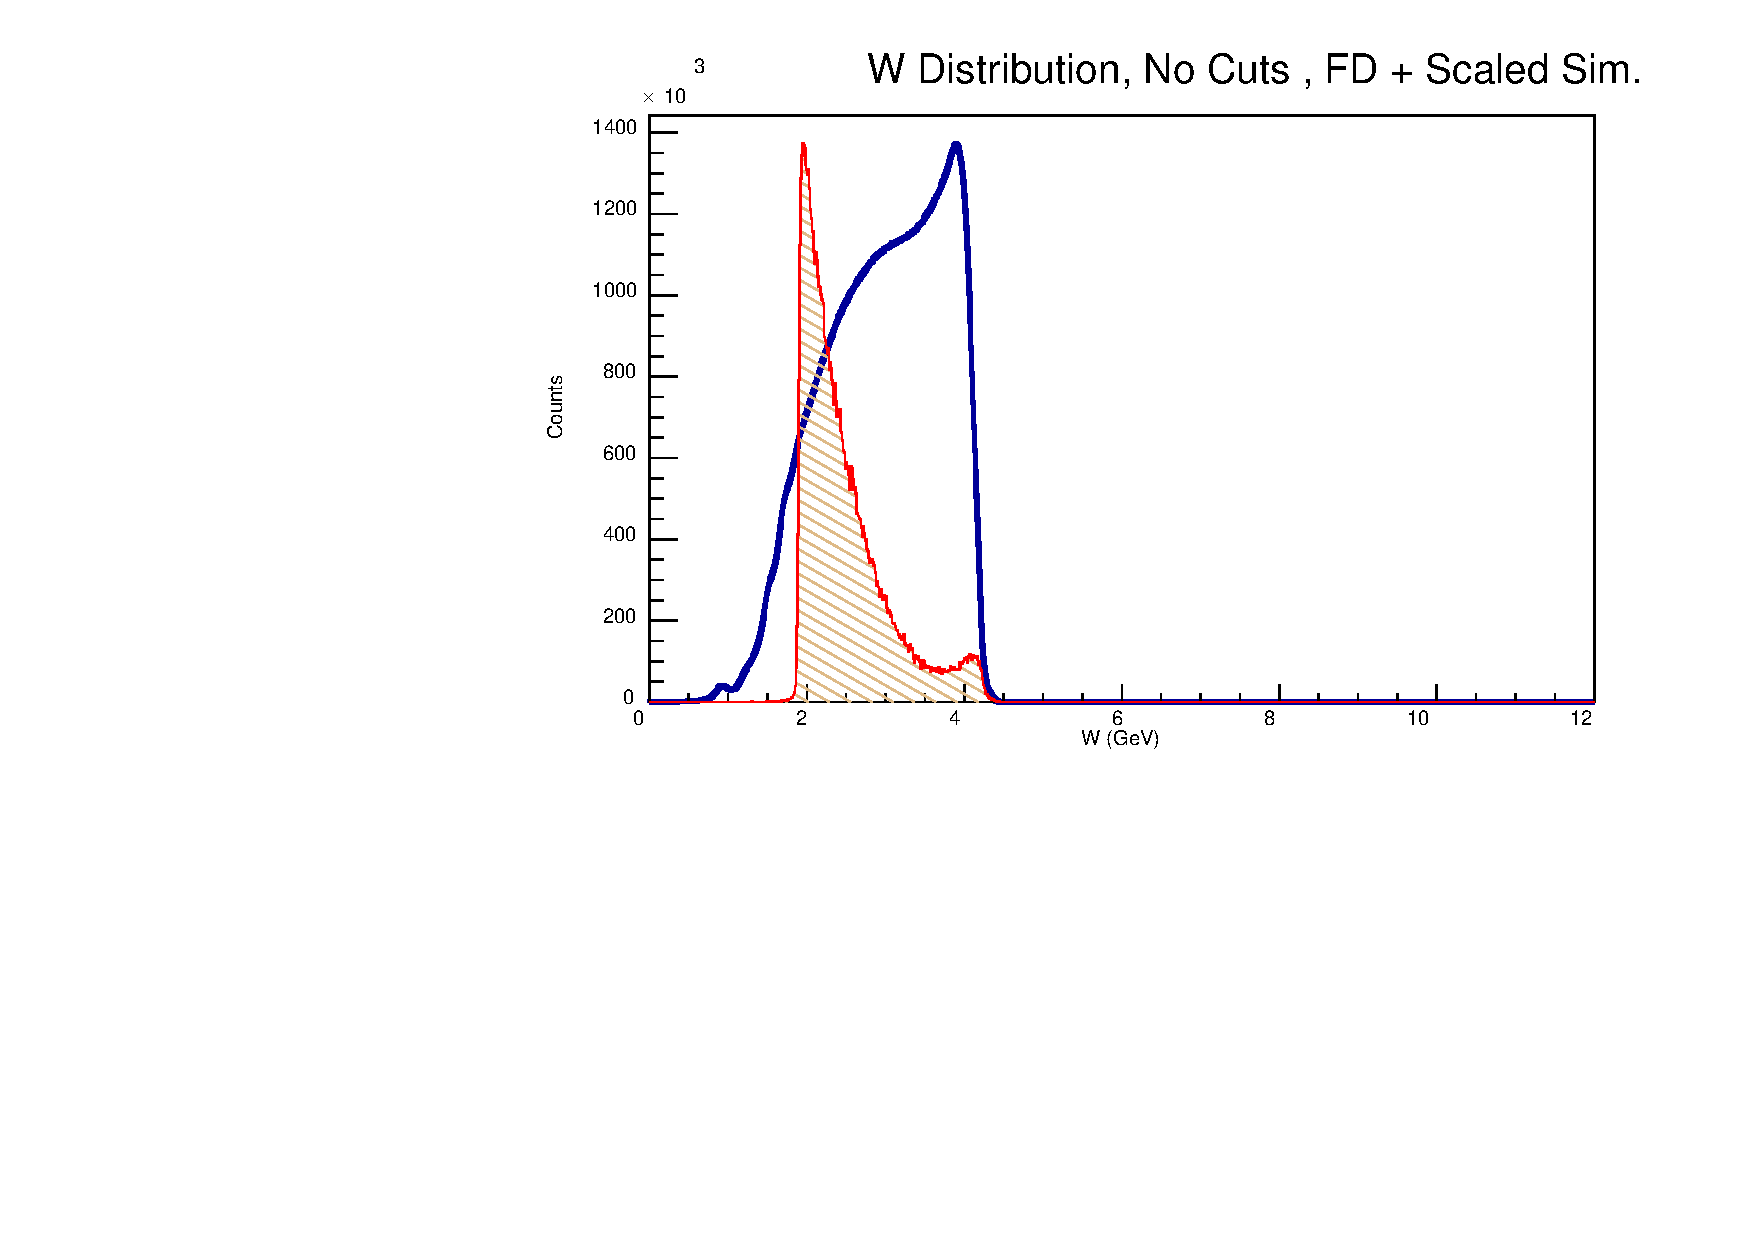
\includegraphics[width=1\textwidth]{figures/Simulation/kinematics_advanced/hist_w_nocut_fd_Double.pdf}
            \end{subfigure}%
            \begin{subfigure}{.5\textwidth}
                \centering
                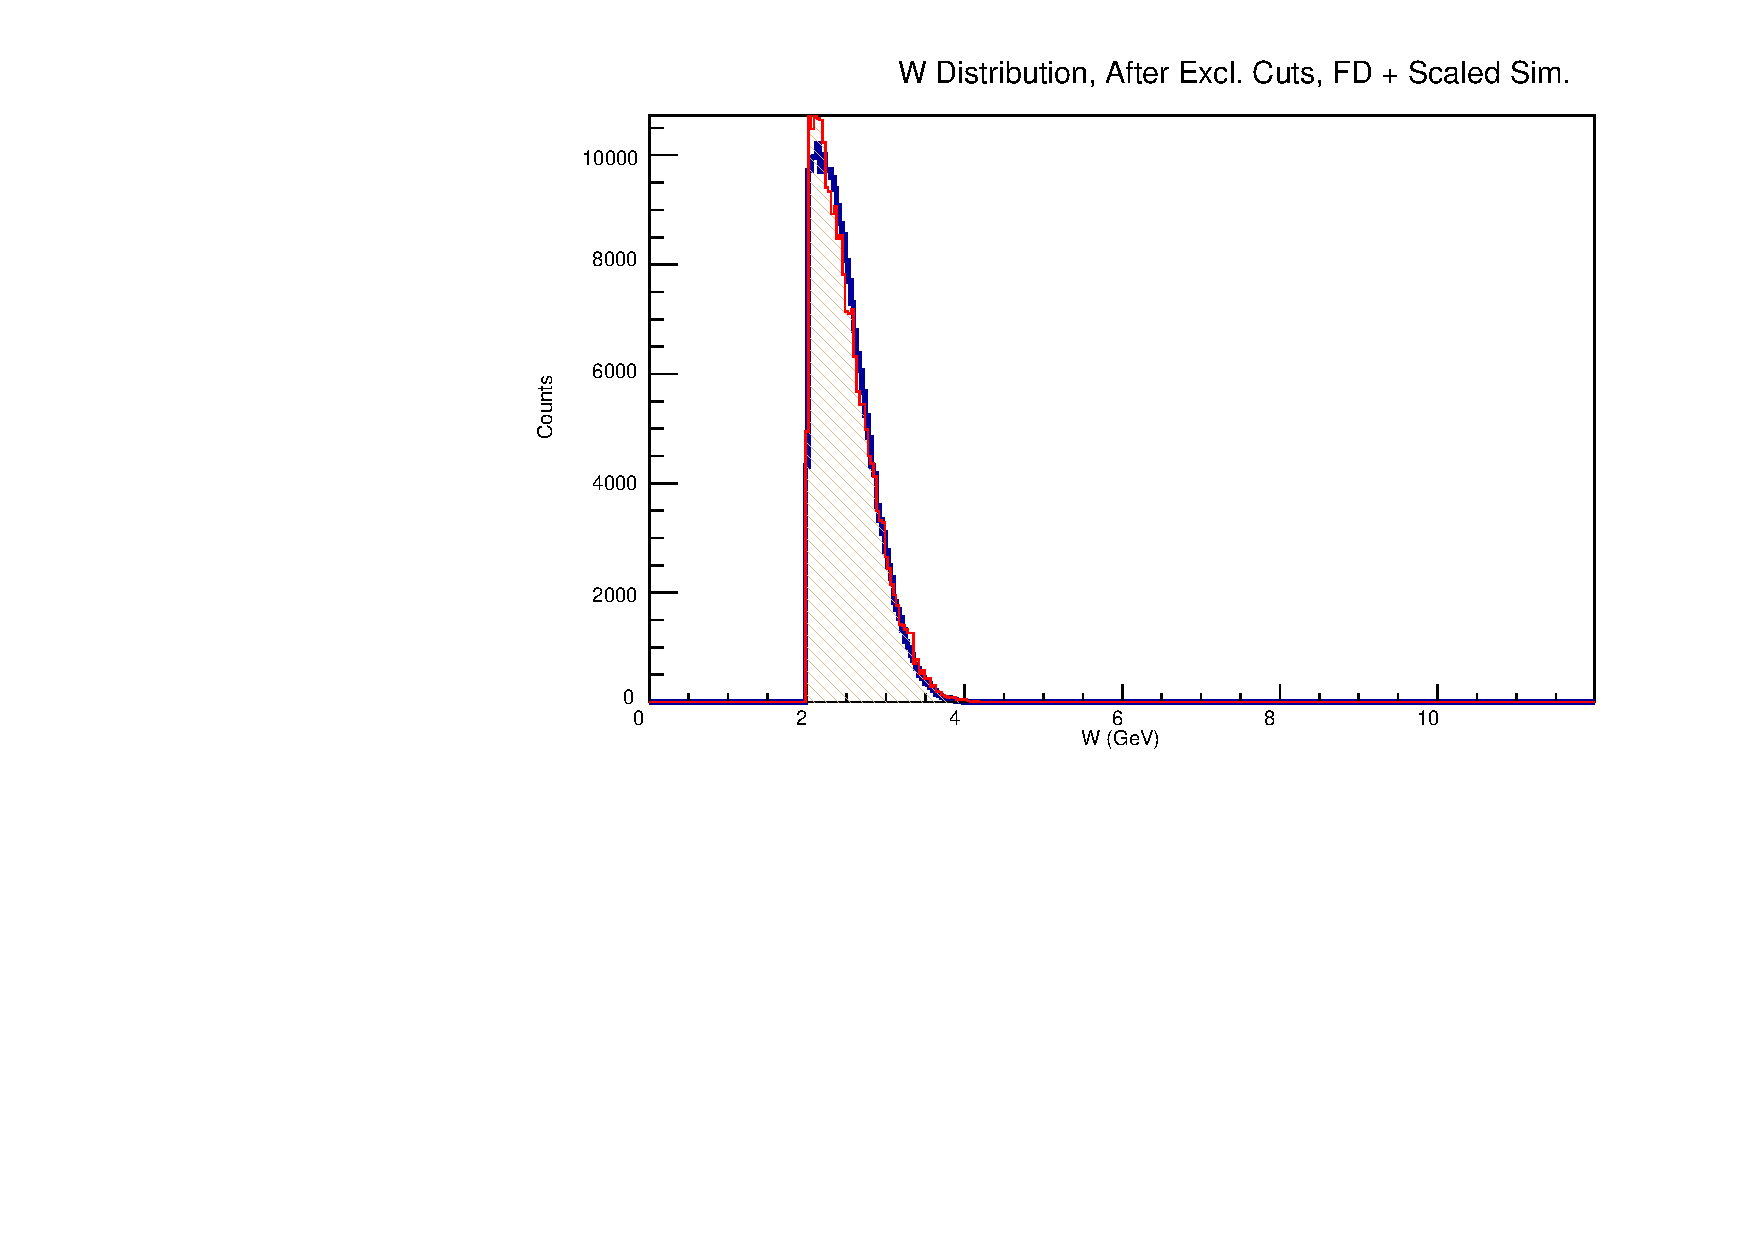
\includegraphics[width=1\textwidth]{figures/Simulation/kinematics_advanced/hist_w_excut_fd_Double.pdf}
            \end{subfigure}
            \begin{subfigure}{.5\textwidth}
                \centering
                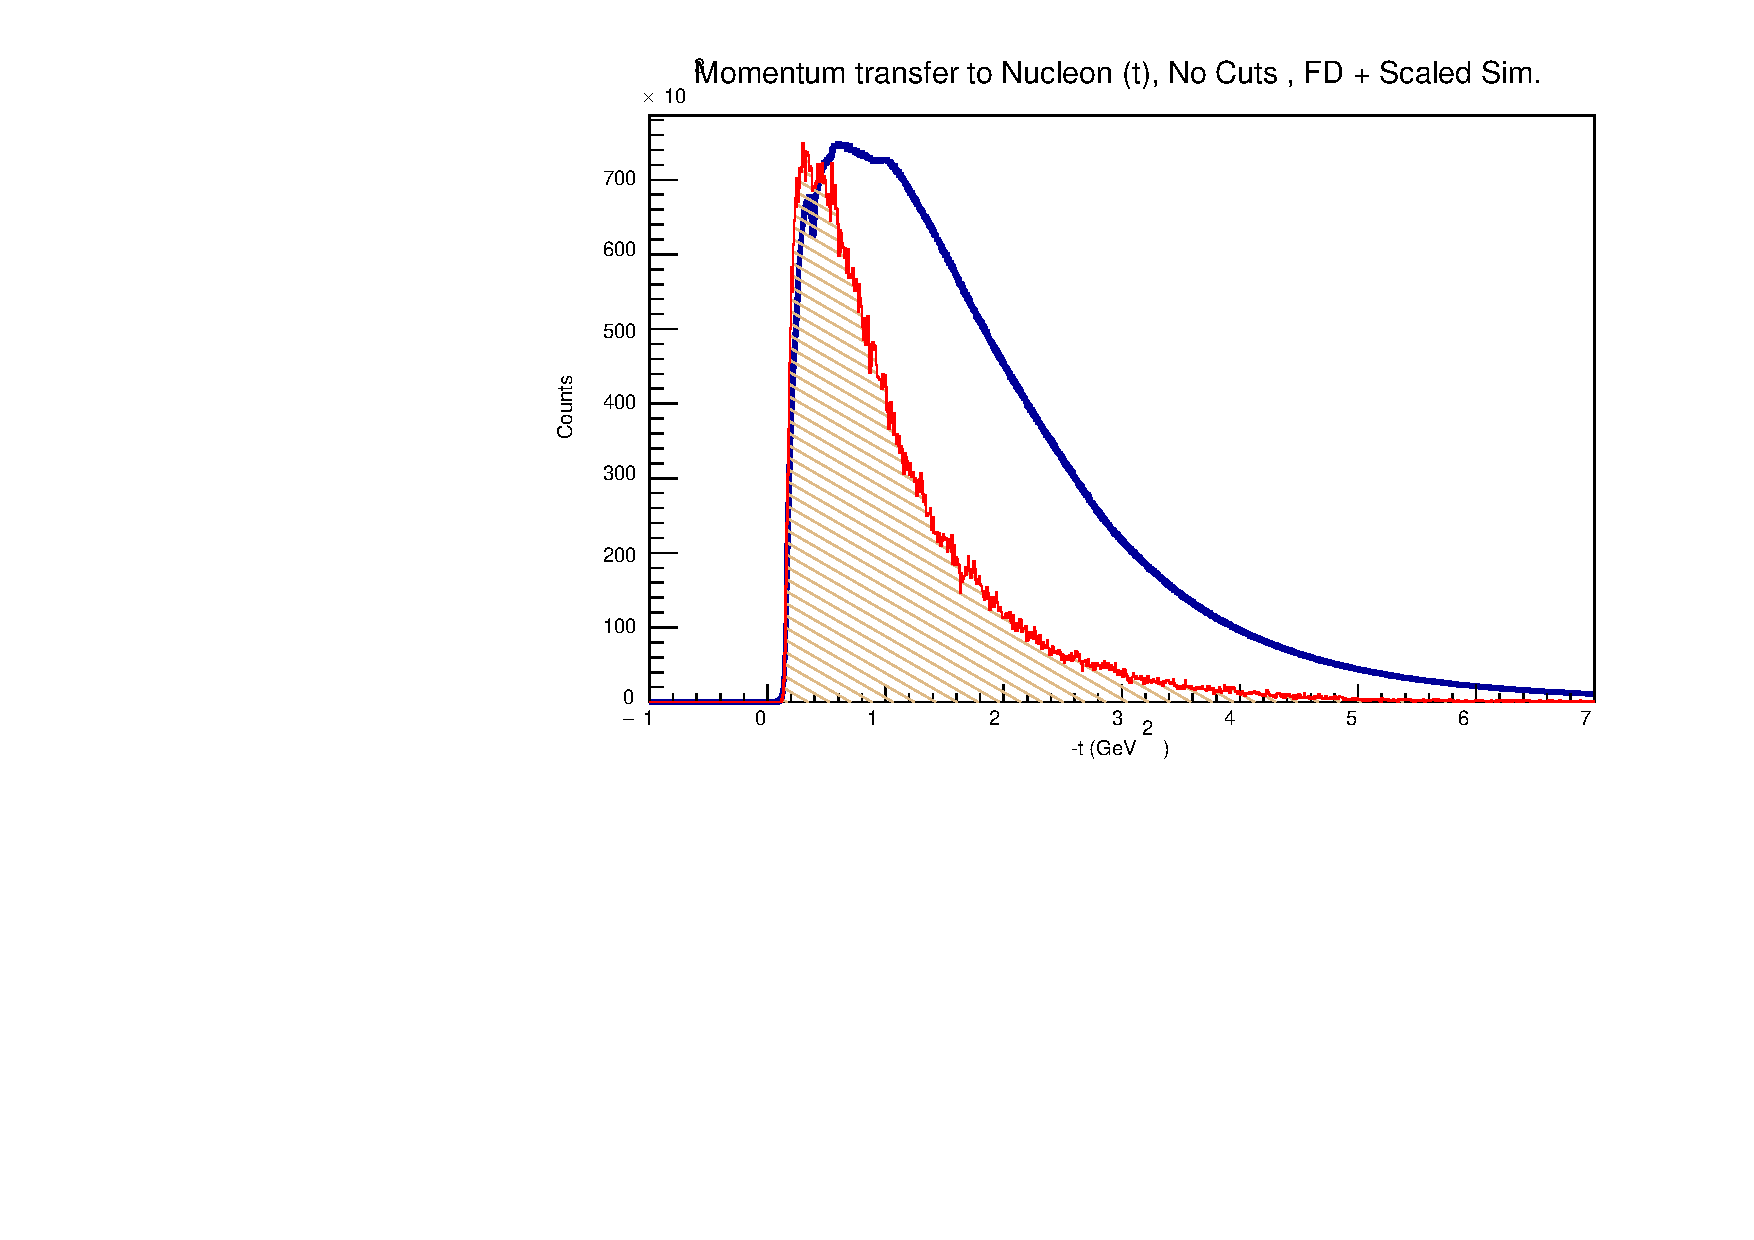
\includegraphics[width=1\textwidth]{figures/Simulation/kinematics_advanced/hist_kinematic_t_nocut_fd_Double.pdf}
            \end{subfigure}%
            \begin{subfigure}{.5\textwidth}
                \centering
                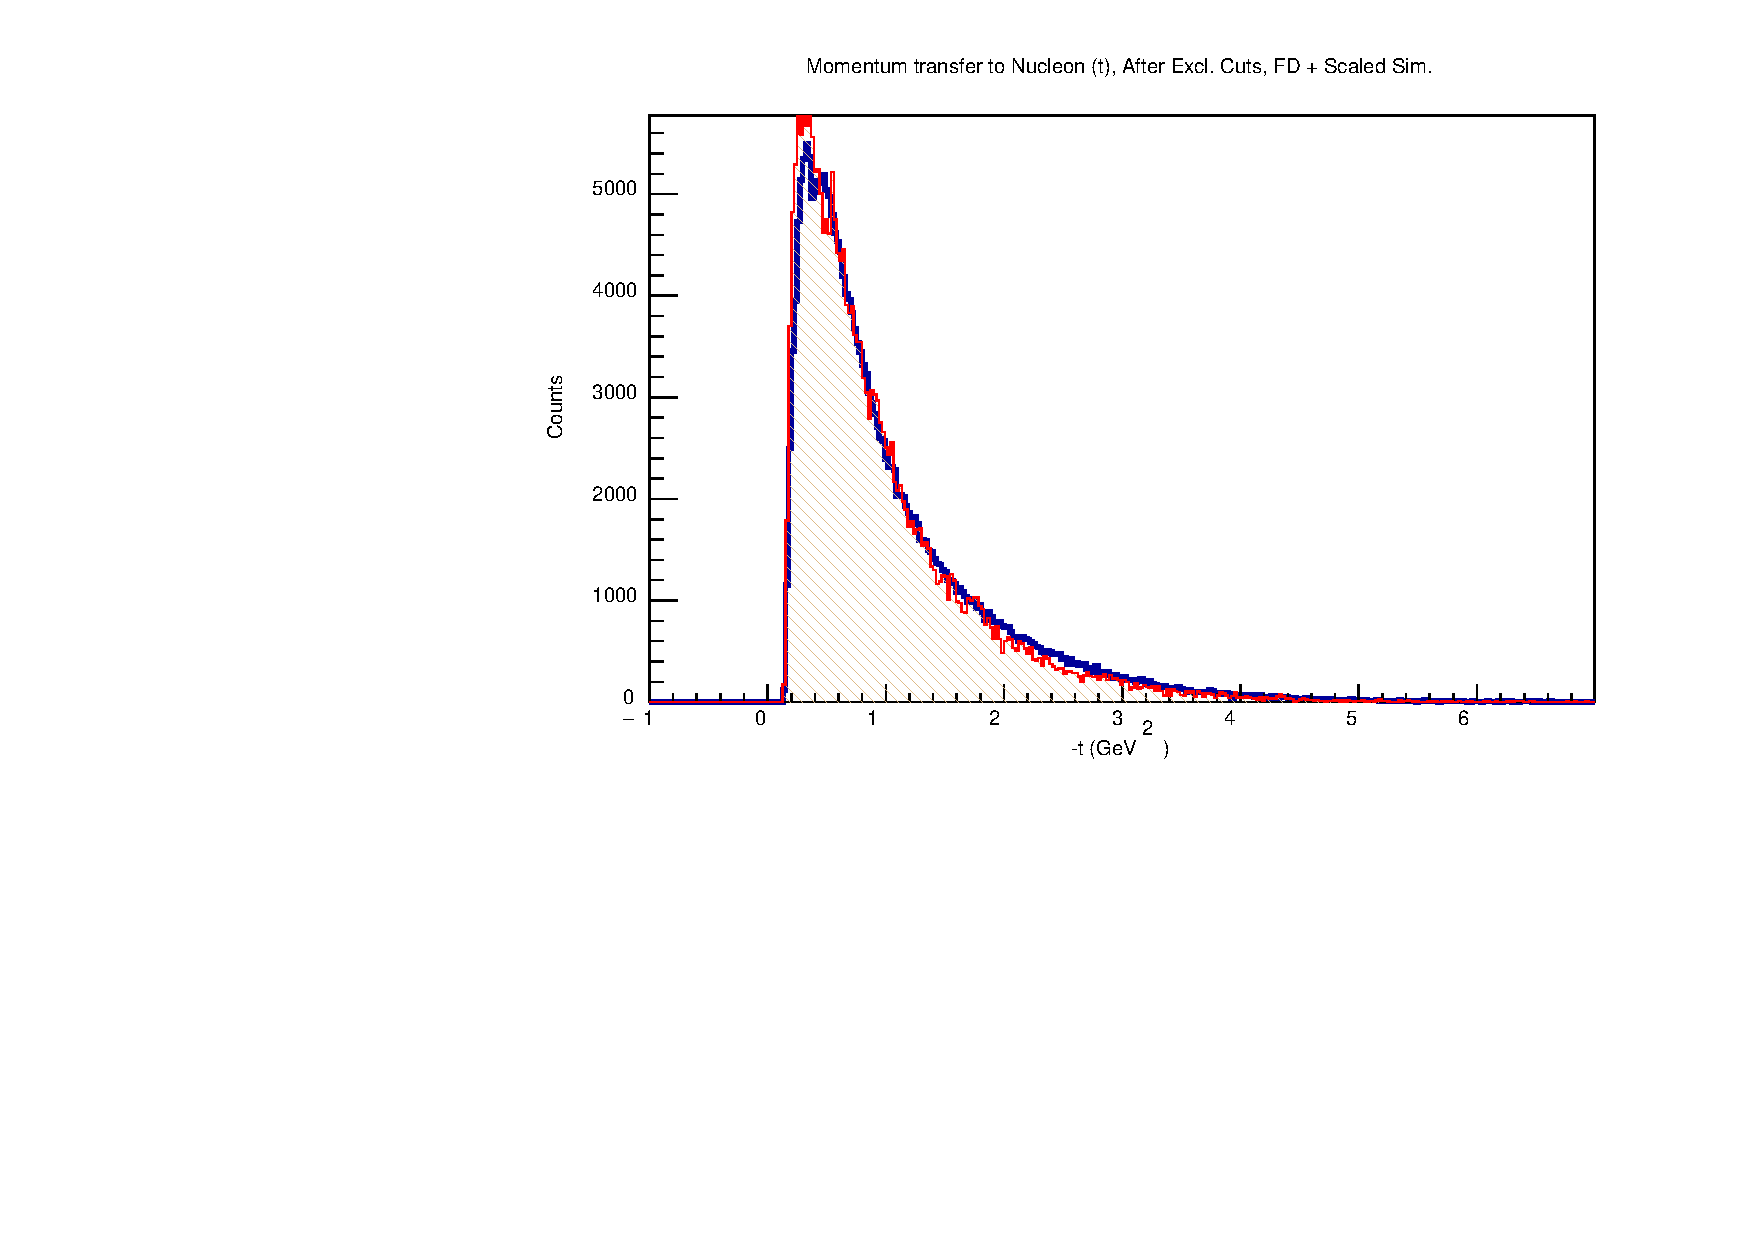
\includegraphics[width=1\textwidth]{figures/Simulation/kinematics_advanced/hist_kinematic_t_excut_fd_Double.pdf}
            \end{subfigure}
            \caption[short]{W (top) and t (bottom) distributions, before exclusivity cuts (left) and after (right) for data (blue) and simulation (red)}
        \end{figure} 
        
    \clearpage


\section{Comparison to Data: Reconstructed Pion and Exclusivity}

    \subsection{Pion Mass and Energy}
    The pion mass distribution shows particularly good overlap between data and simulation, indicating that the method of reconstruction for pions is performing well.

        \begin{figure}[!htb]
            \centering
            \begin{subfigure}{.5\textwidth}
                \centering
                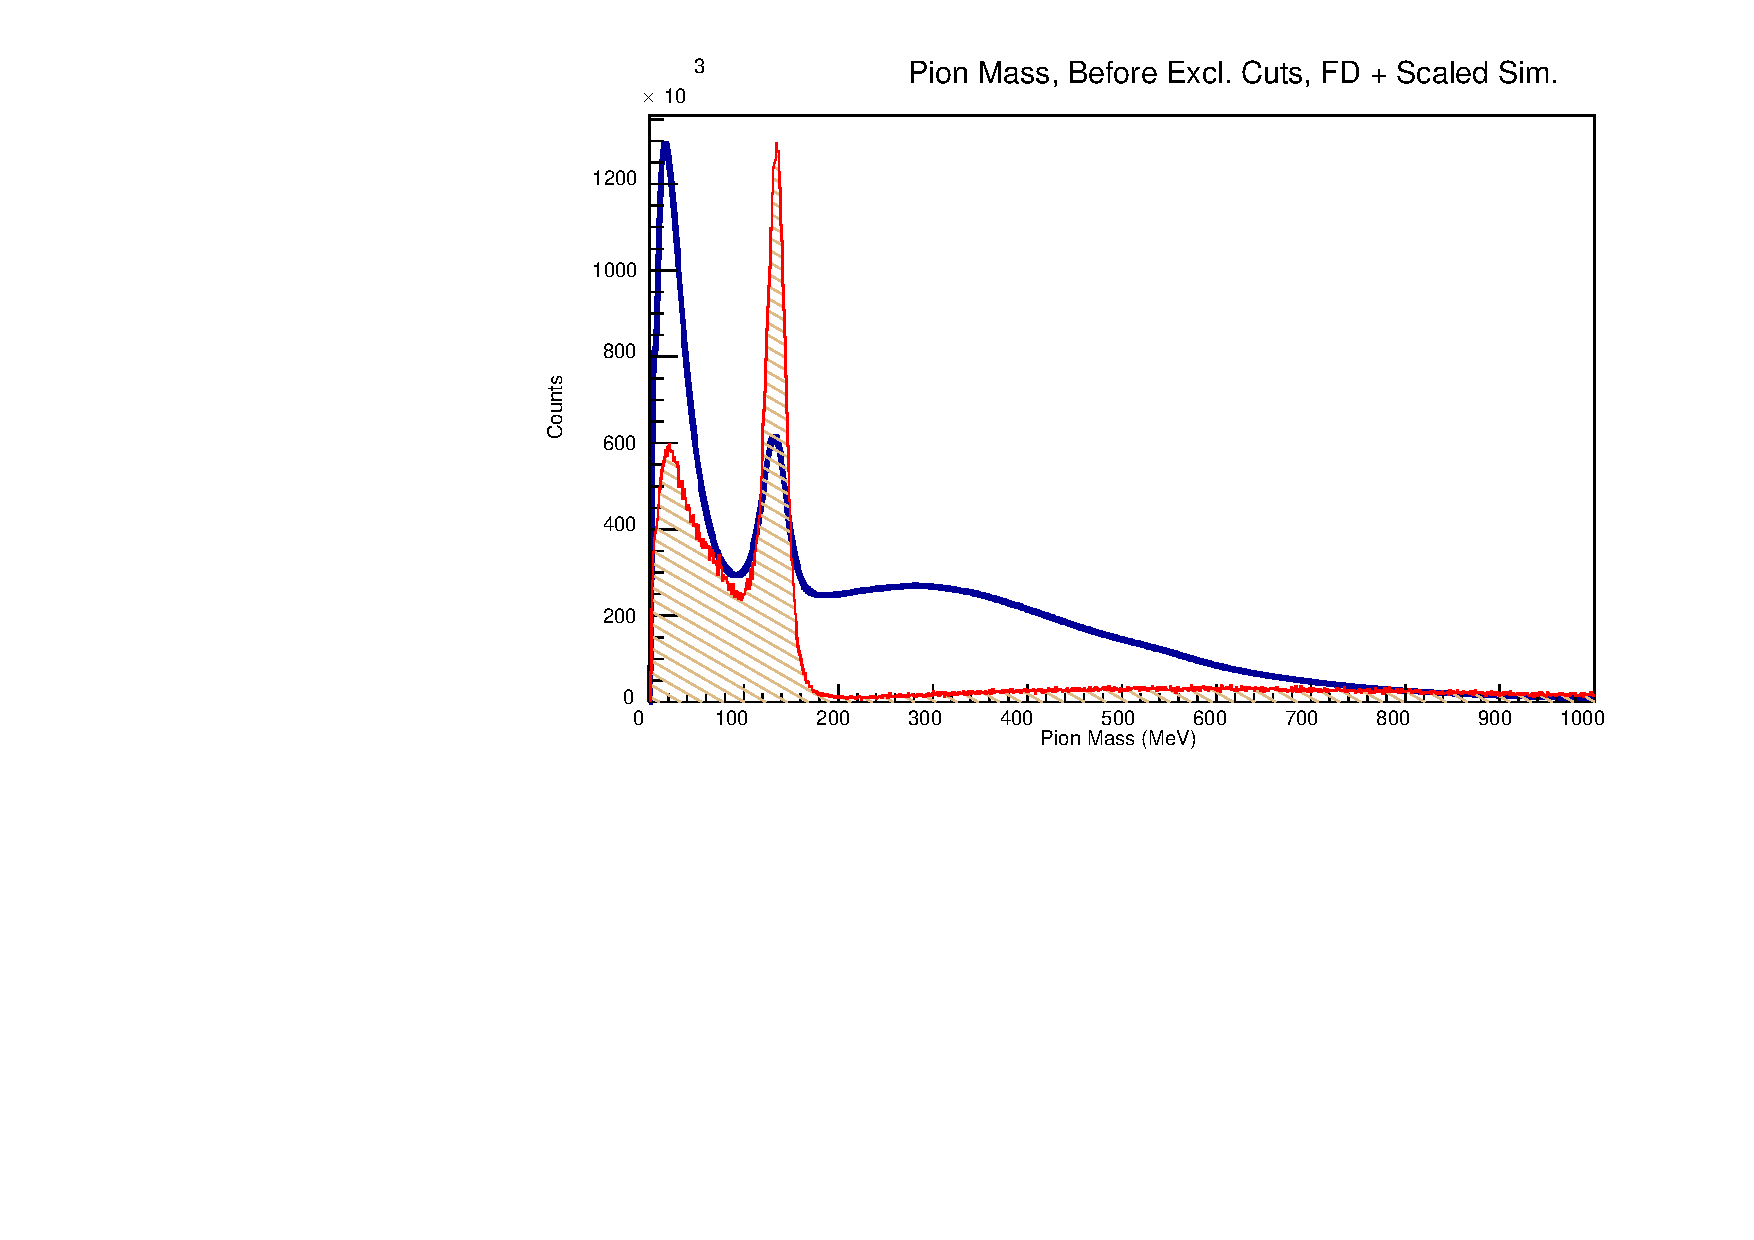
\includegraphics[width=1\textwidth]{figures/Simulation/exclusivity/hist_pion_mass_prexcut_fd_Double.pdf}
            \end{subfigure}%
            \begin{subfigure}{.5\textwidth}
                \centering
                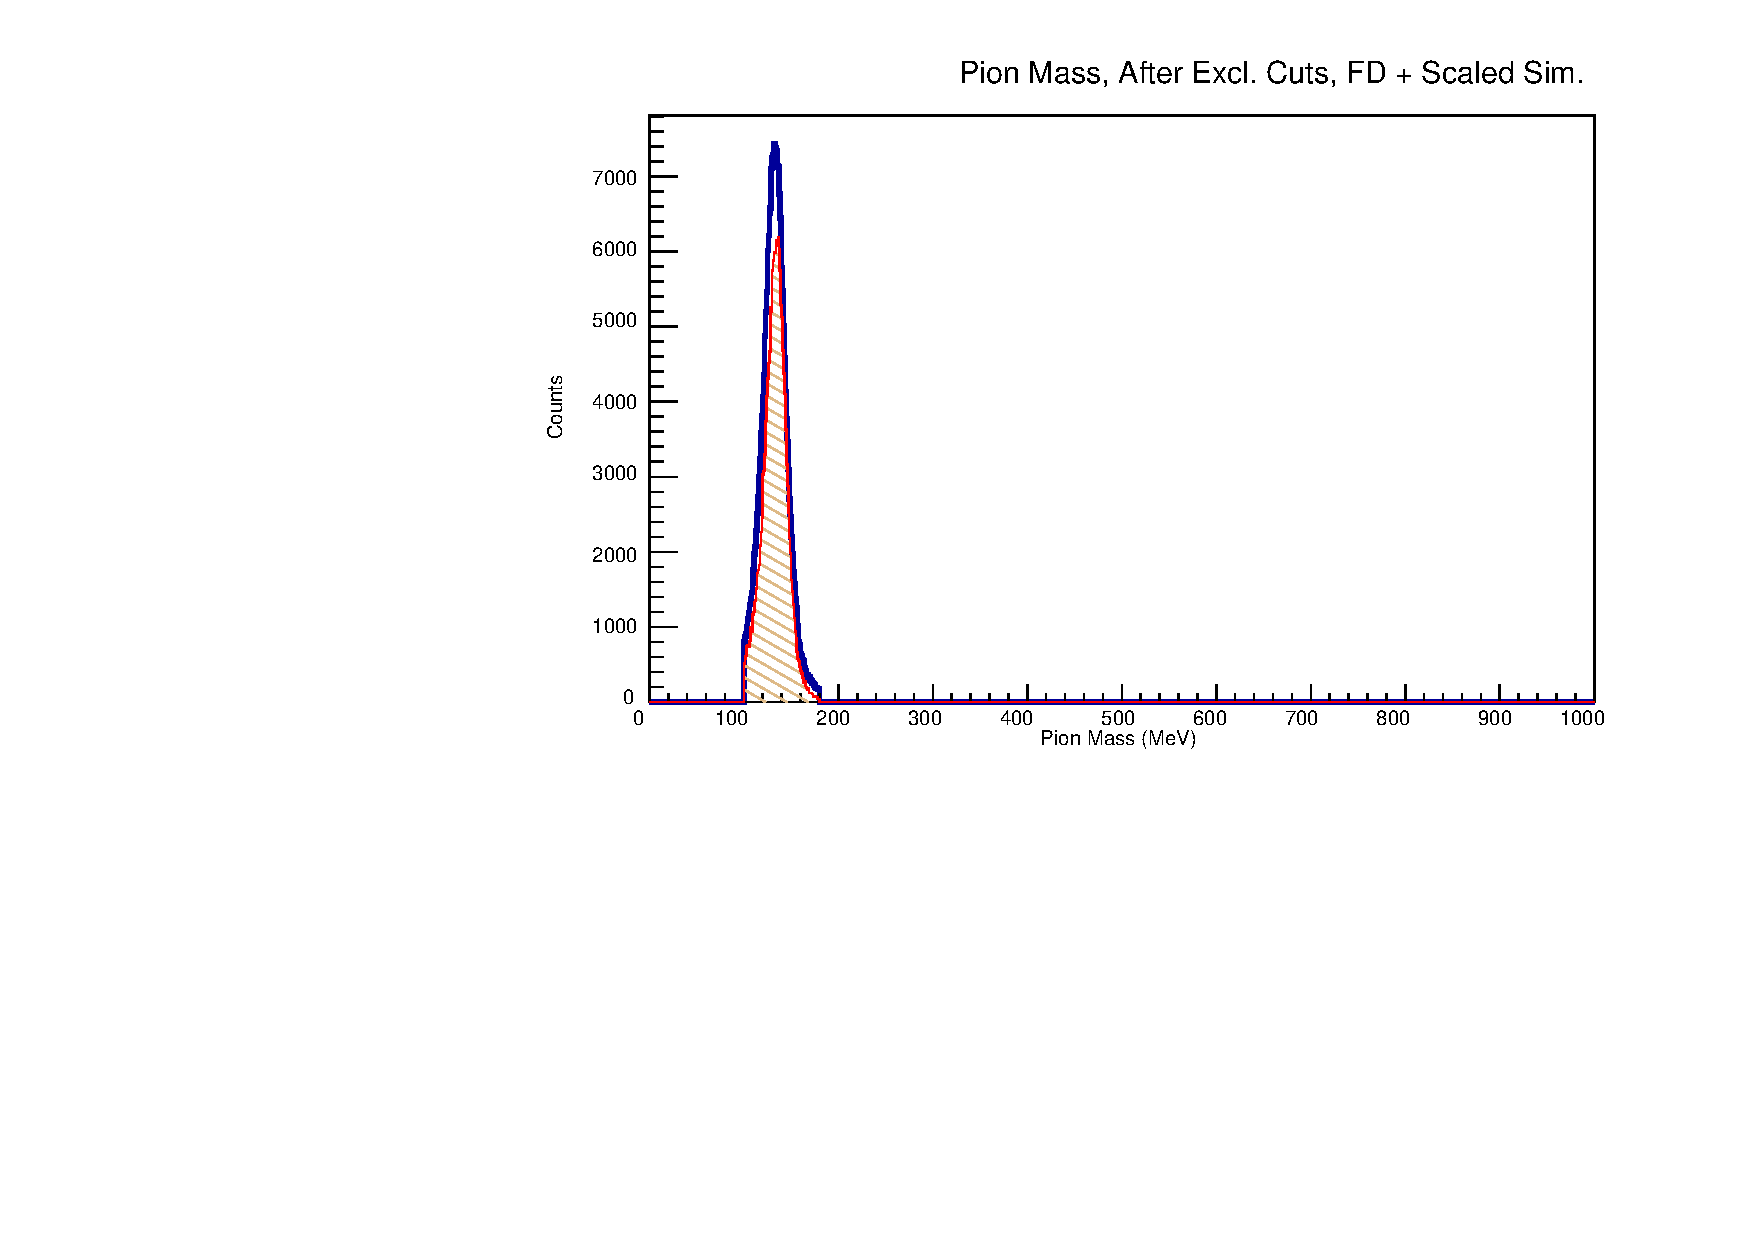
\includegraphics[width=1\textwidth]{figures/Simulation/exclusivity/hist_pion_mass_excut_fd_Double.pdf}
            \end{subfigure}
            \begin{subfigure}{.5\textwidth}
                \centering
                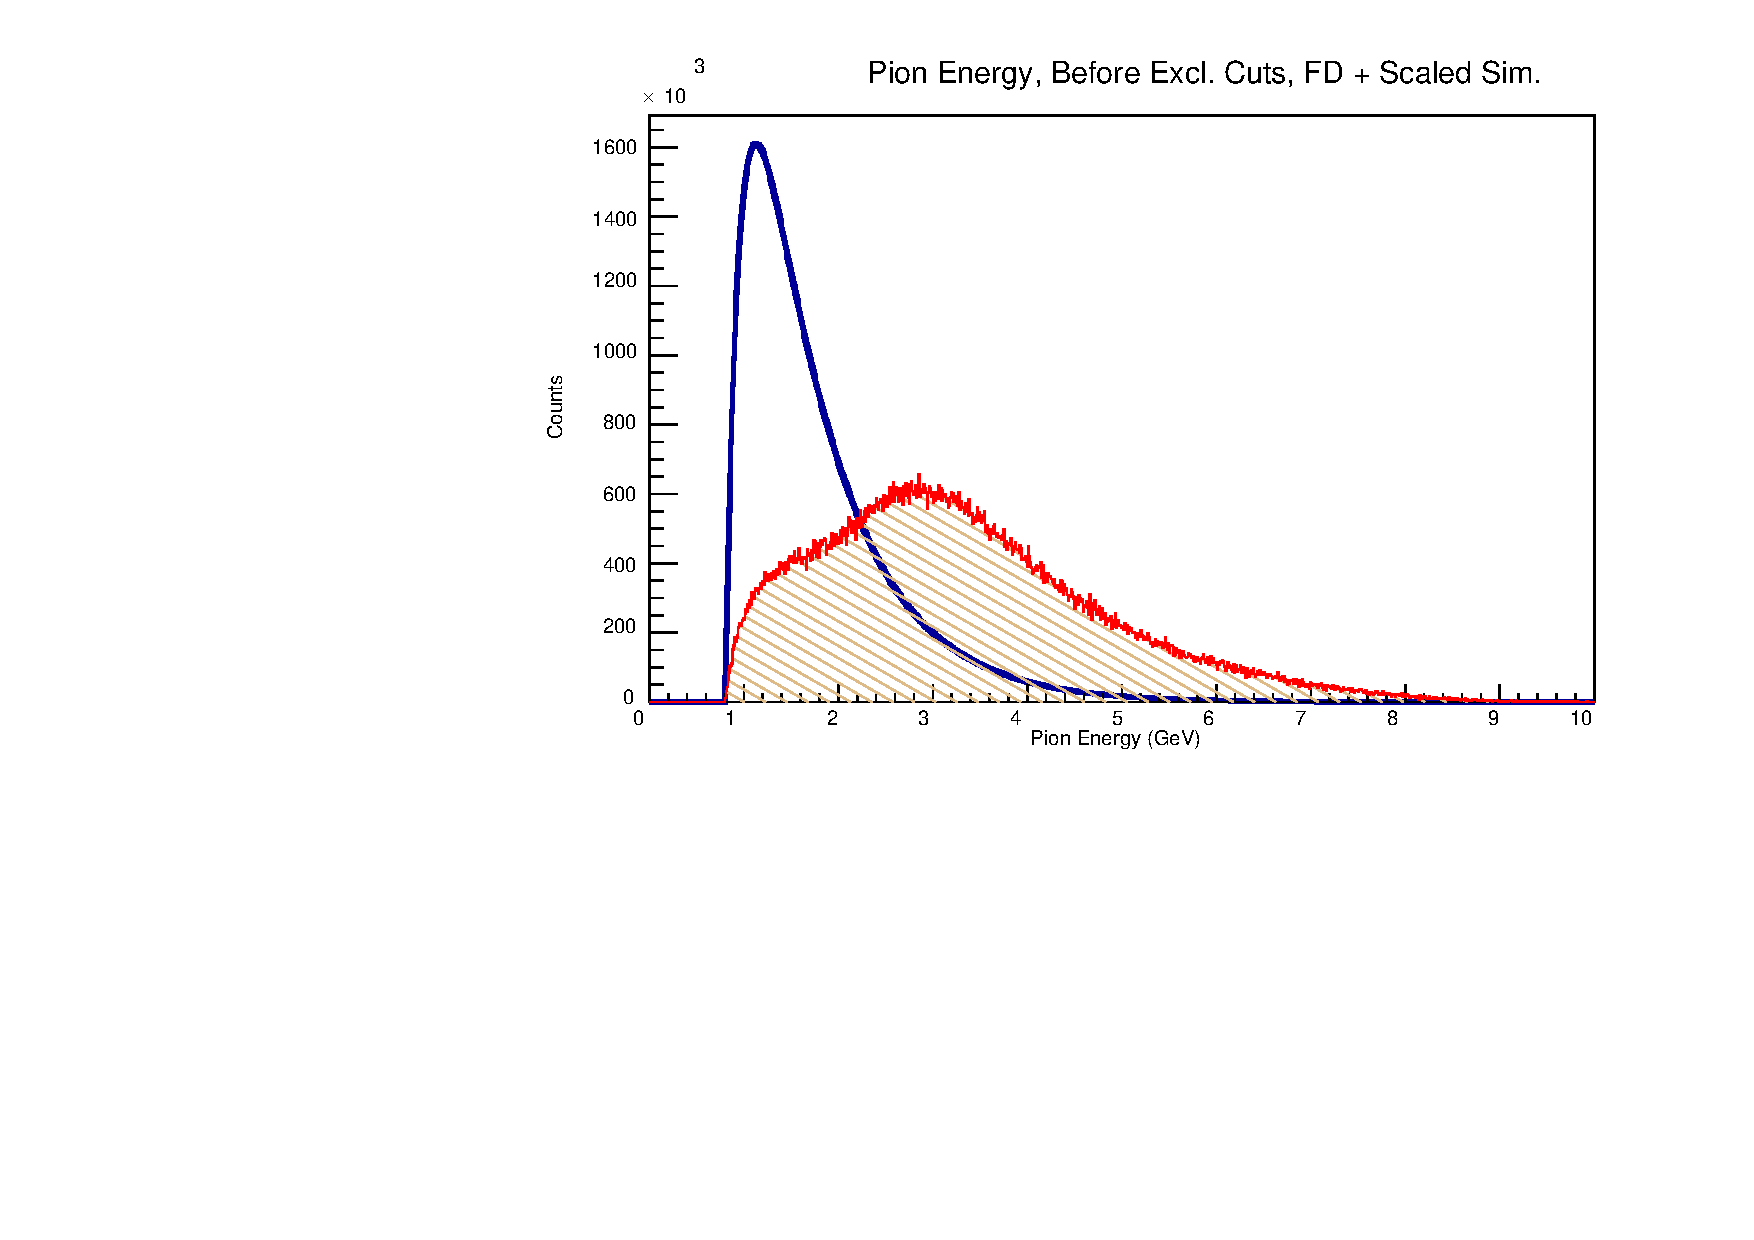
\includegraphics[width=1\textwidth]{figures/Simulation/exclusivity/hist_pion_energy_prexcut_fd_Double.pdf}
            \end{subfigure}%
            \begin{subfigure}{.5\textwidth}
                \centering
                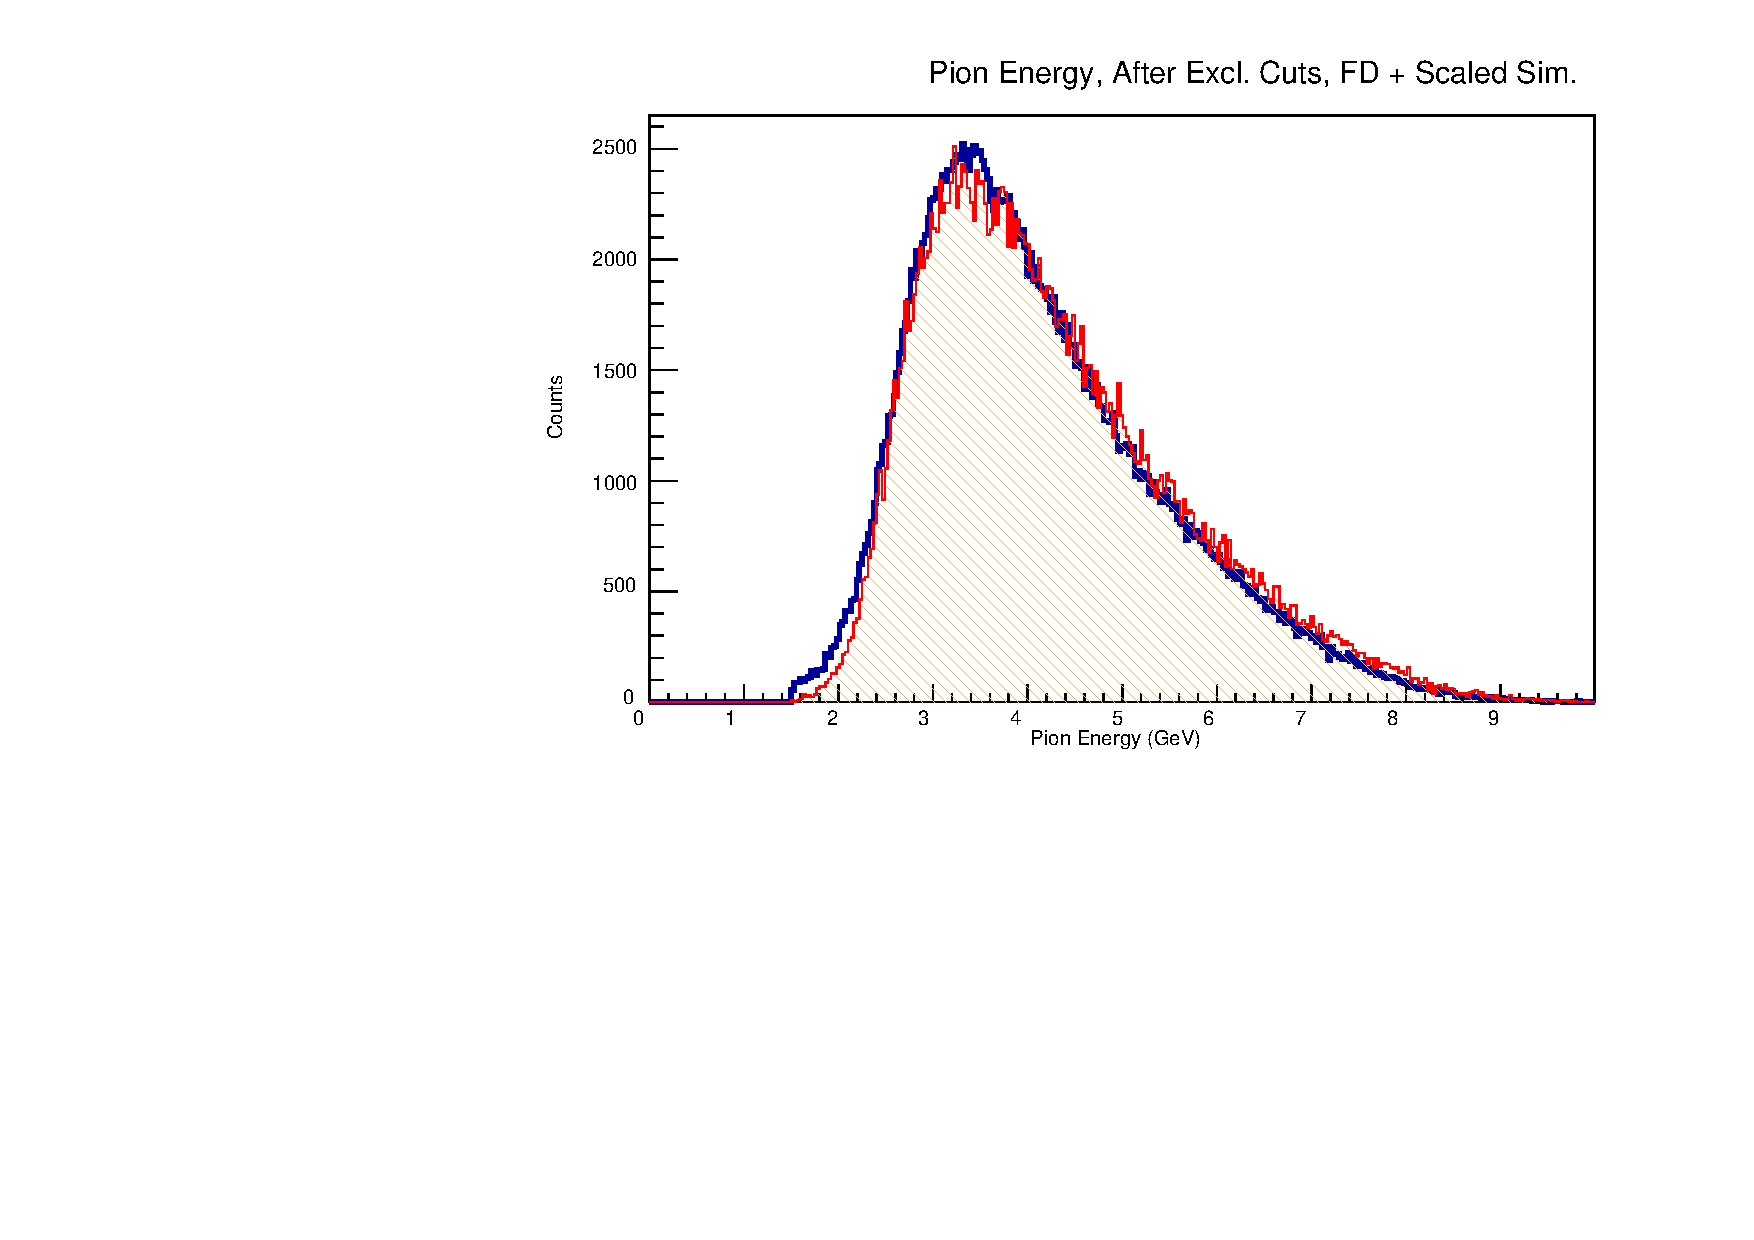
\includegraphics[width=1\textwidth]{figures/Simulation/exclusivity/hist_pion_energy_excut_fd_Double.pdf}
            \end{subfigure}
            \caption[short]{Pion mass (top) and energy (bottom) distributions, before exclusivity cuts (left) and after (right) for data (blue) and simulation (red)}
        \end{figure}

    \clearpage

    \subsection{Missing Mass}
    Figure \ref{fig:MM} shows missing mass distributions for (epX) and (ep$\gamma \gamma$) systems. (epX) is calculated by summing the four-momenta of the incoming electron and proton, and subtracting the four-momenta of the outgoing electron and proton. For an exclusive $ep\pi^0$ event, the missing mass squared of (epX) should equal just the $\pi^0$ mass squared, 0.02 GeV$^2$. (ep$\gamma \gamma$) is calculated similarly; summing the four-momenta of the incoming electron and proton, and subtracting the four-momenta of the outgoing electron, proton, and two photons constituting the candidate reconstructed $\pi^0$. For an exclusive event, the missing mass should be exactly zero. In both cases, the data and simulation are close to the expected value, and show a high degree of overlap.
    

        \begin{figure}[!htb]
            \centering
            \begin{subfigure}{.45\textwidth}
                \centering
                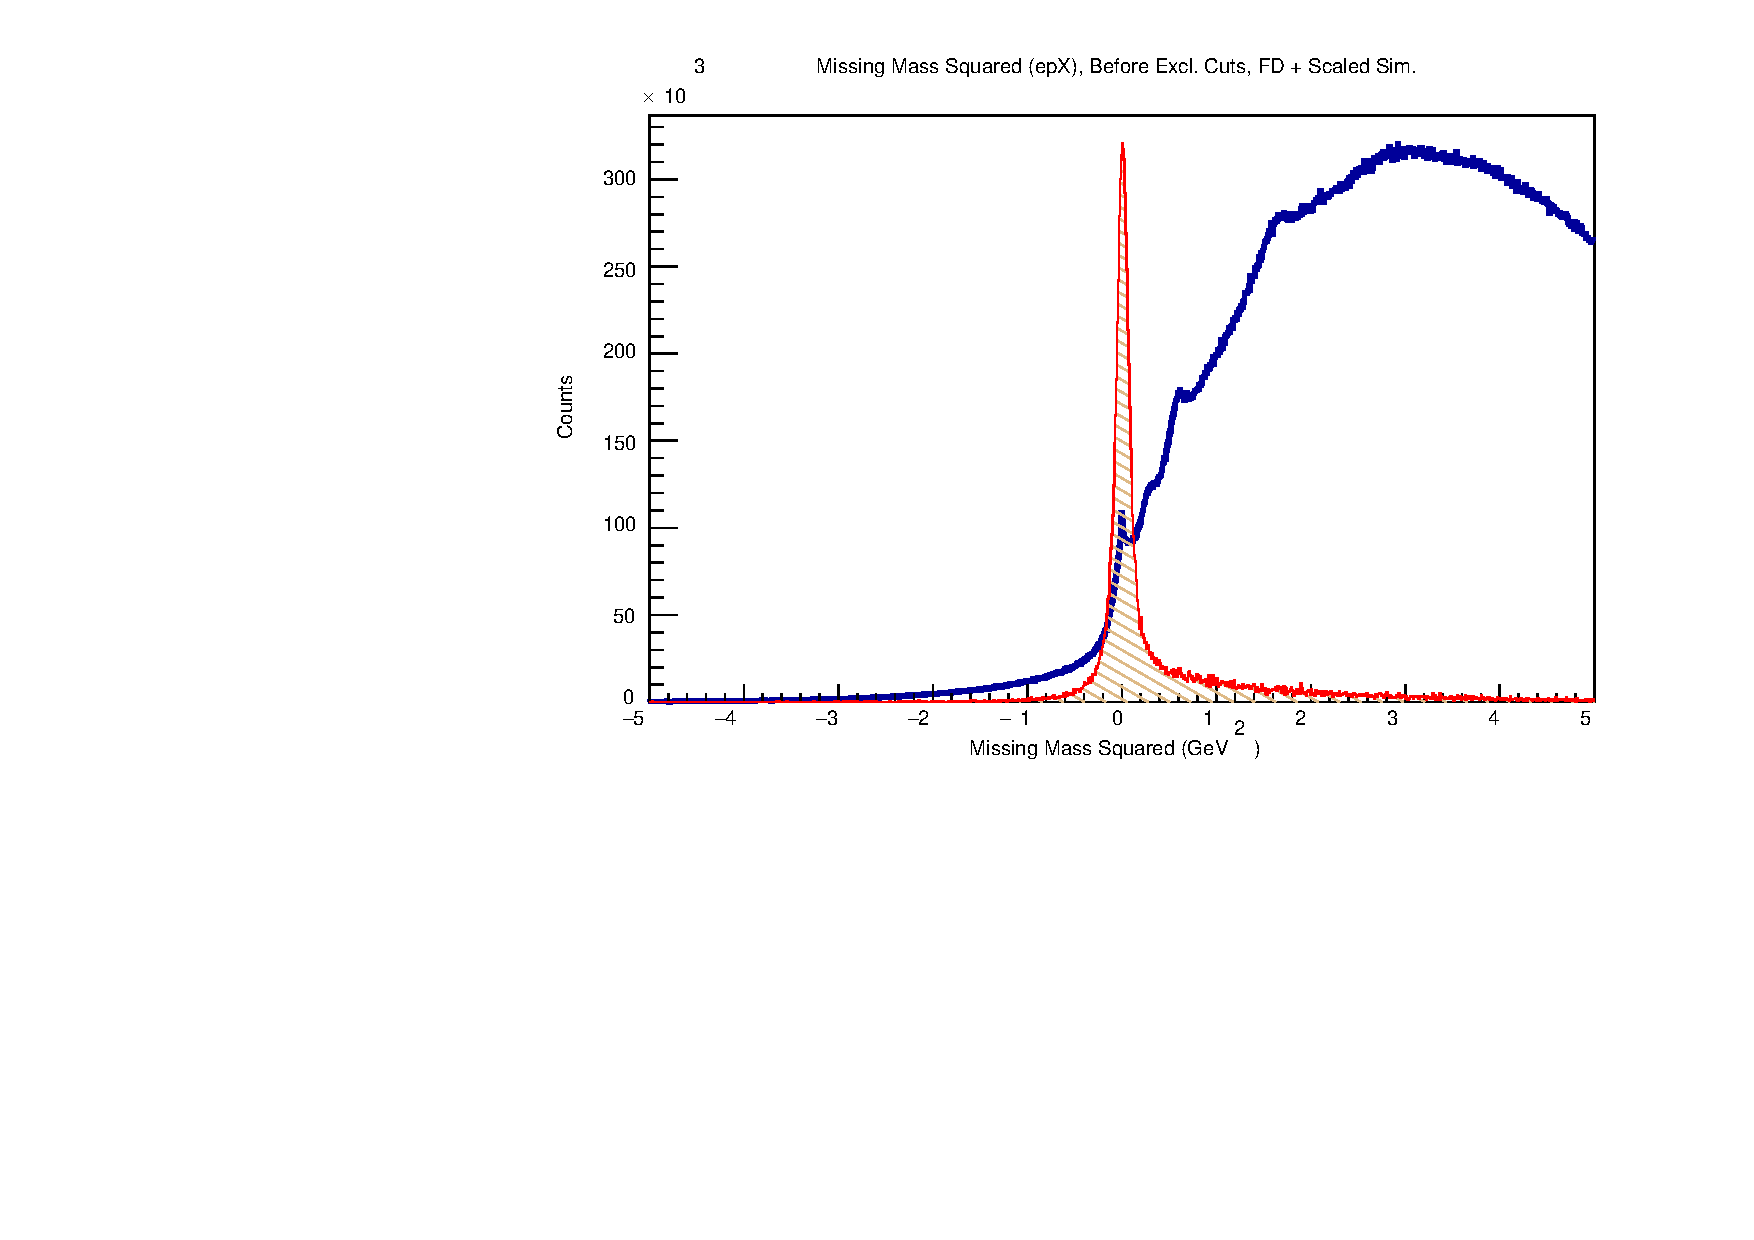
\includegraphics[width=1\textwidth]{figures/Simulation/exclusivity/hist_missing_mass_squared_epX_prexcut_fd_Double.pdf}
            \end{subfigure}%
            \begin{subfigure}{.45\textwidth}
                \centering
                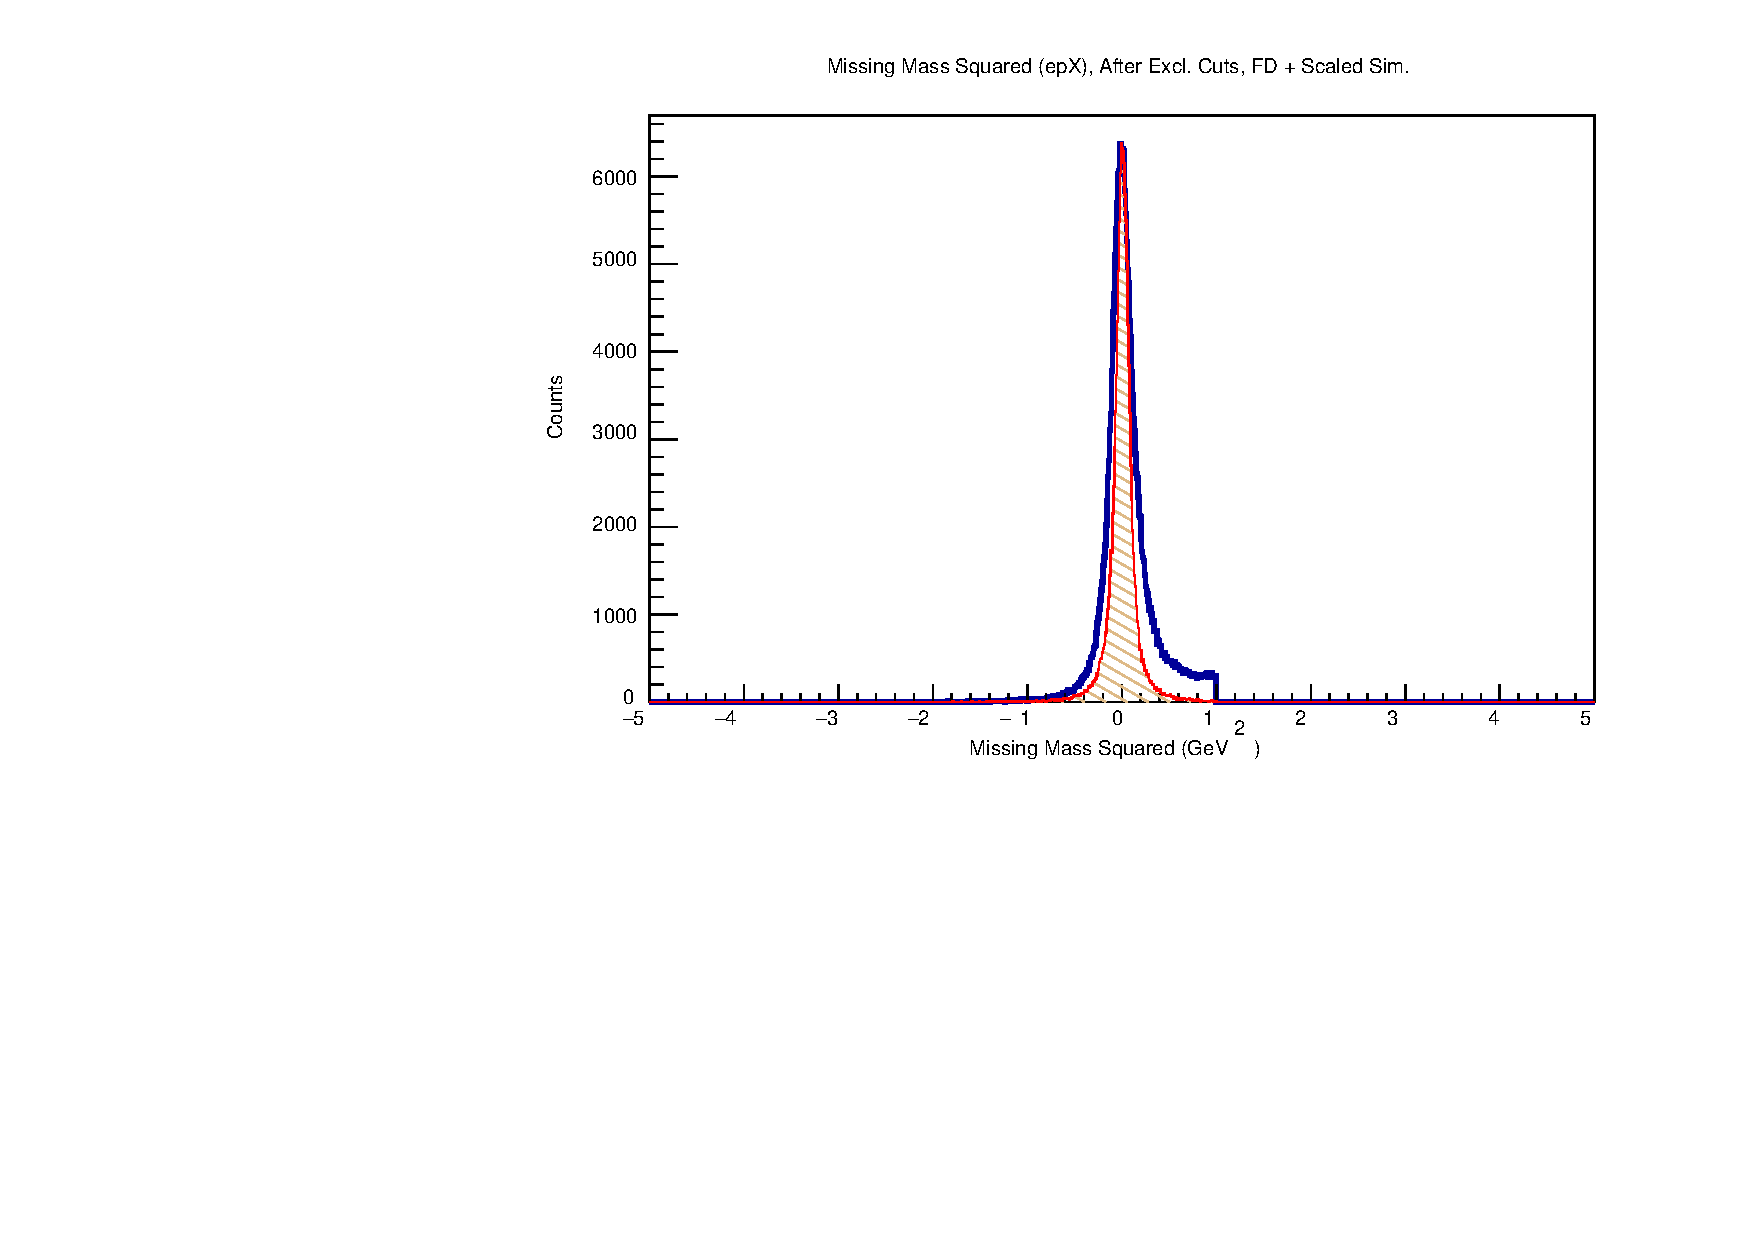
\includegraphics[width=1\textwidth]{figures/Simulation/exclusivity/hist_missing_mass_squared_epX_excut_fd_Double.pdf}
            \end{subfigure}
            \begin{subfigure}{.45\textwidth}
                \centering
                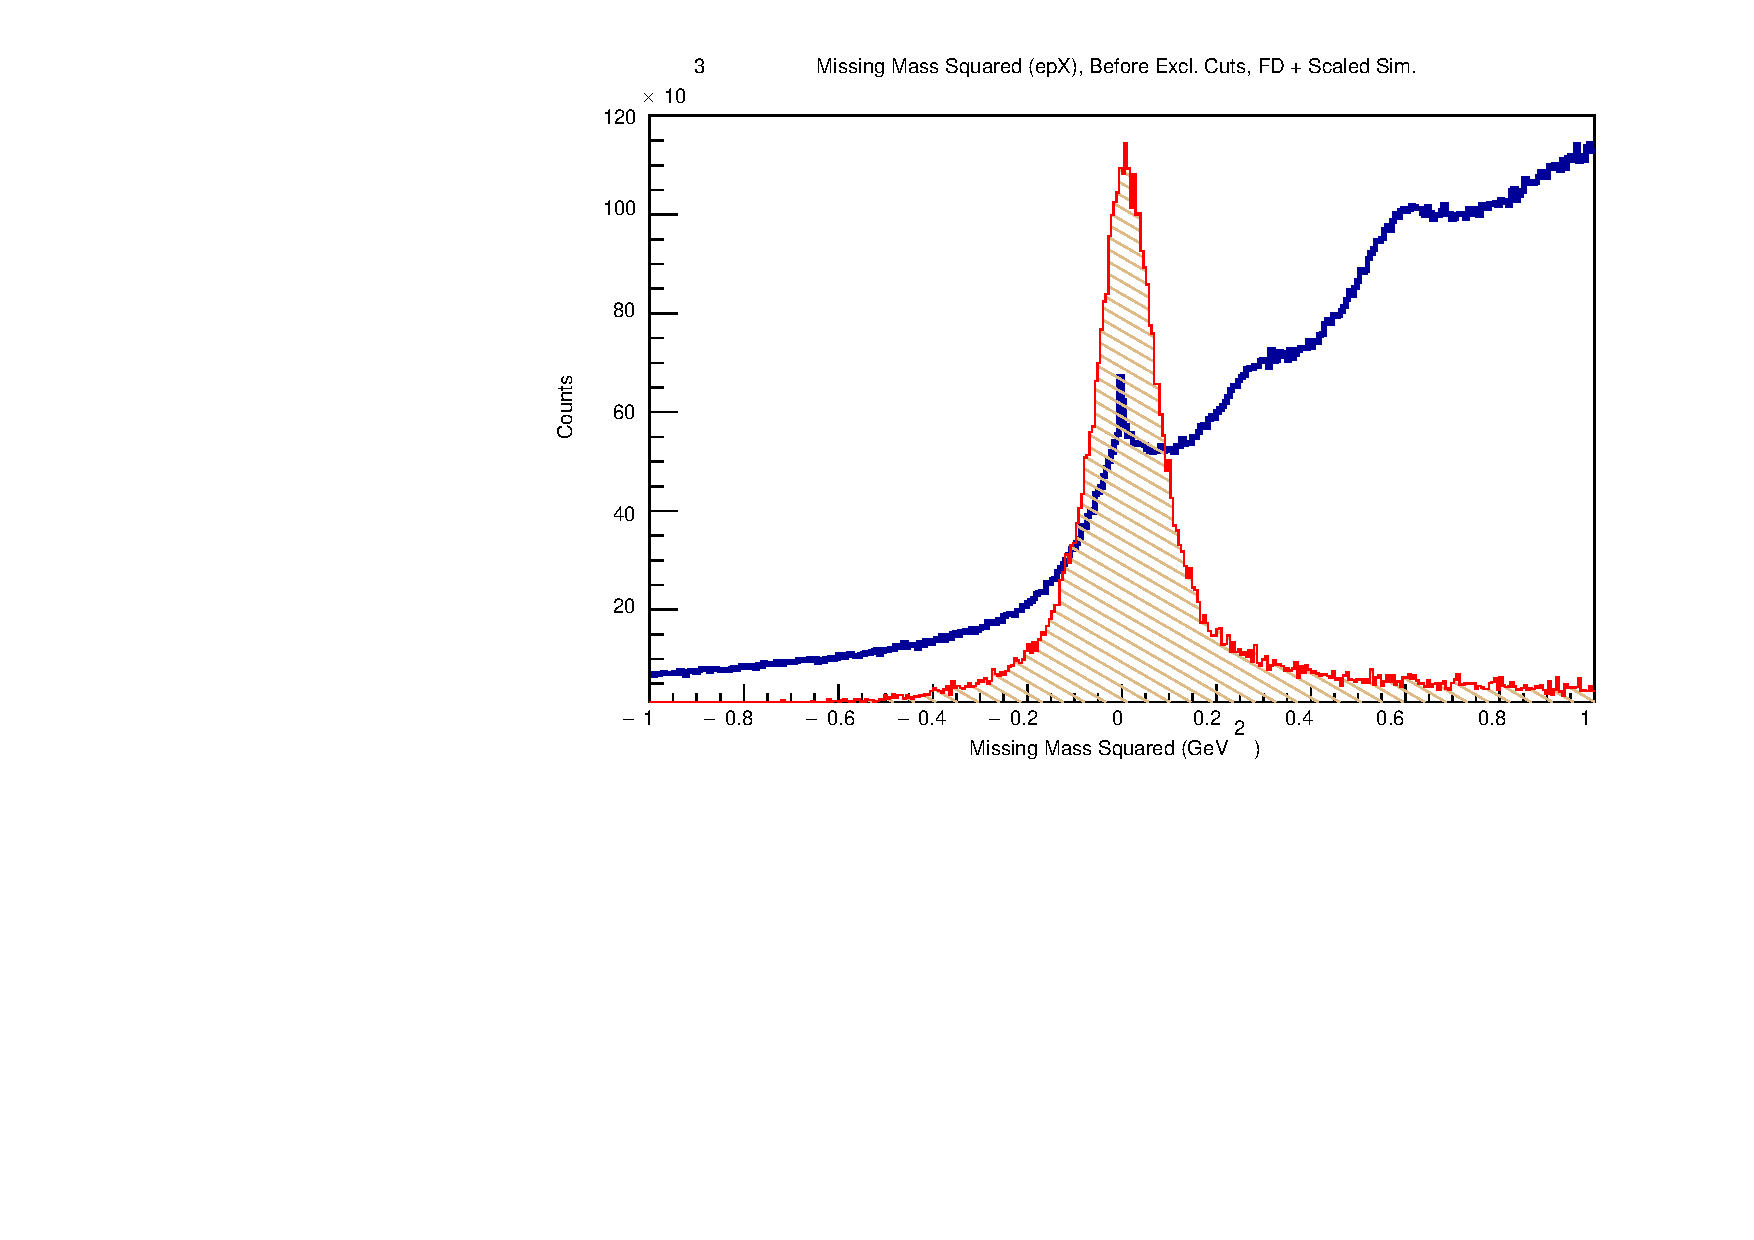
\includegraphics[width=1\textwidth]{figures/Simulation/exclusivity/hist_missing_mass_squared_epX_zoomed_prexcut_fd_Double.pdf}
            \end{subfigure}%
            \begin{subfigure}{.45\textwidth}
                \centering
                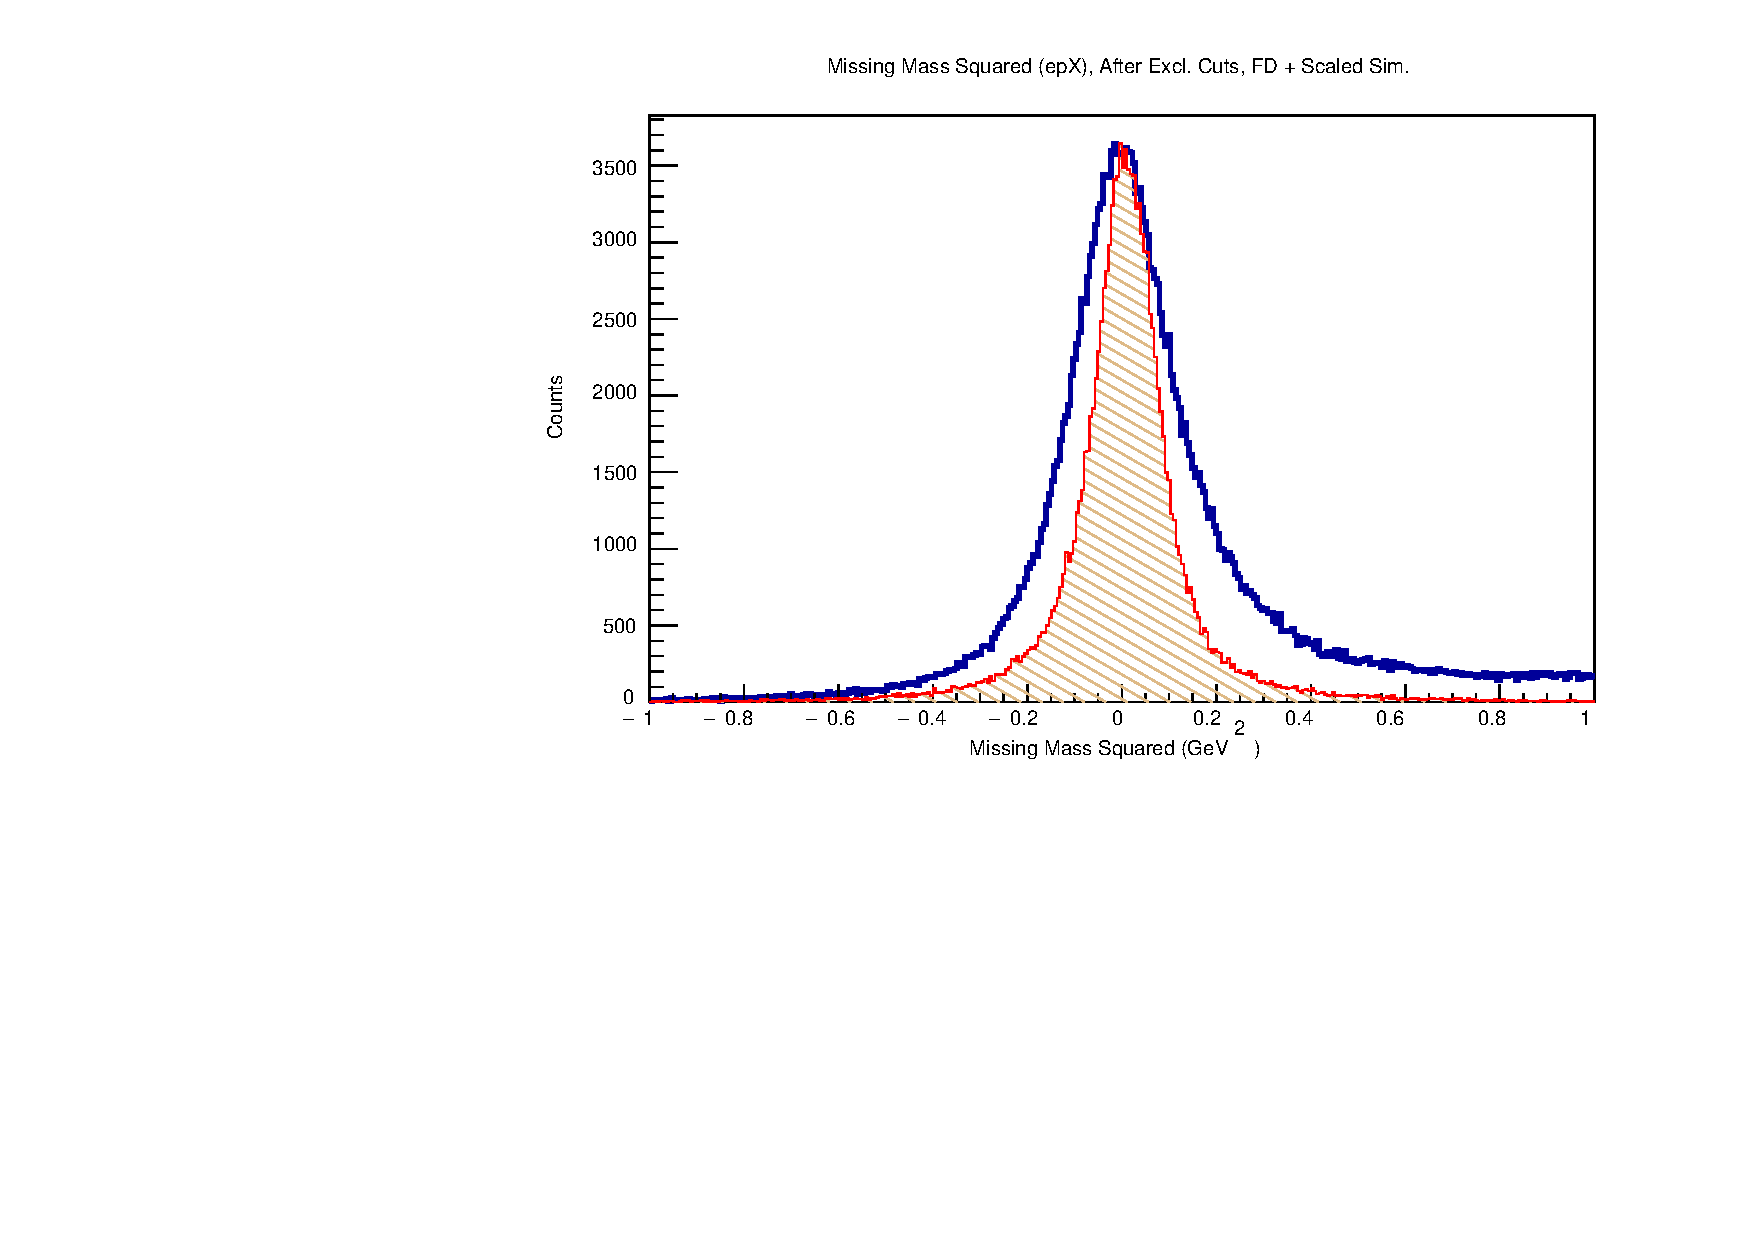
\includegraphics[width=1\textwidth]{figures/Simulation/exclusivity/hist_missing_mass_squared_epX_zoomed_excut_fd_Double.pdf}
            \end{subfigure}
            \begin{subfigure}{.45\textwidth}
                \centering
                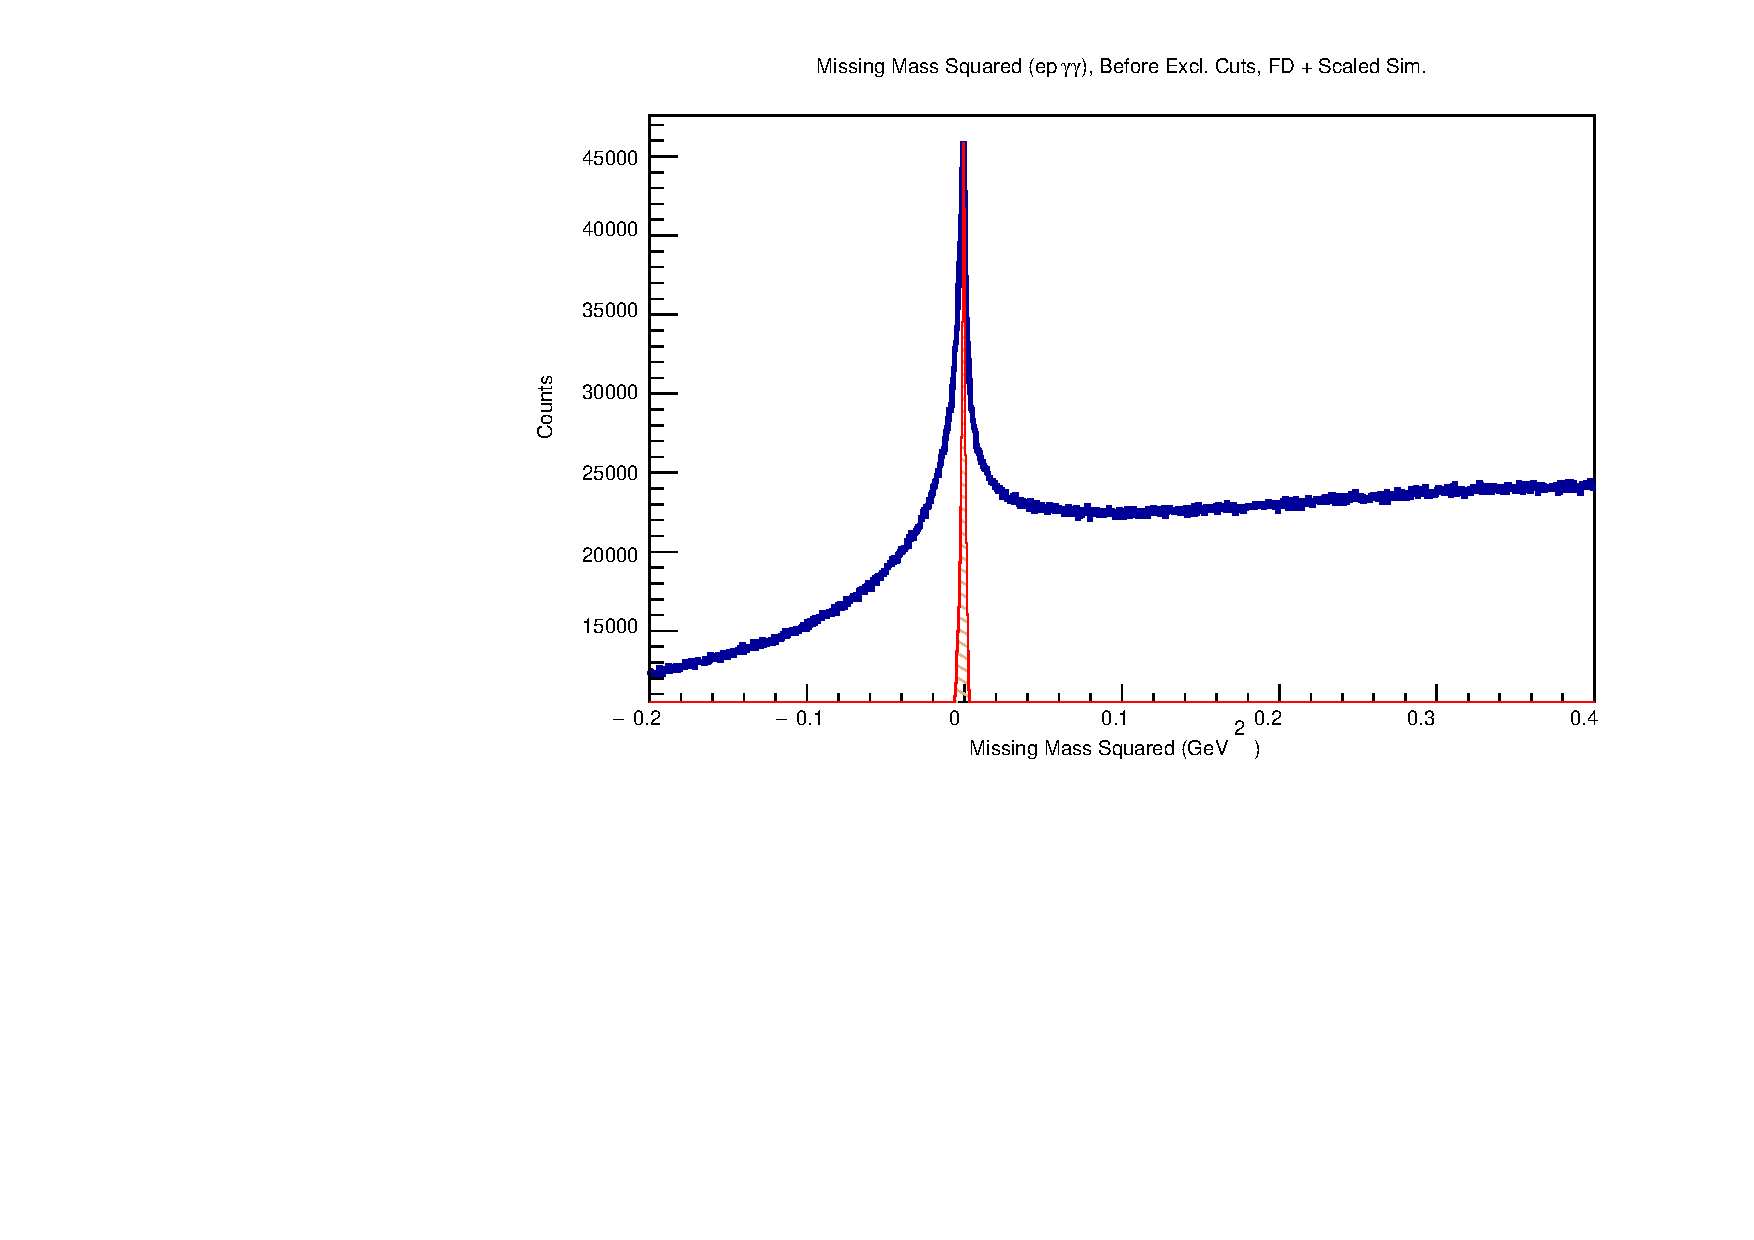
\includegraphics[width=1\textwidth]{figures/Simulation/exclusivity/hist_missing_mass_squared_epgg_prexcut_fd_Double.pdf}
            \end{subfigure}%
            \begin{subfigure}{.45\textwidth}
                \centering
                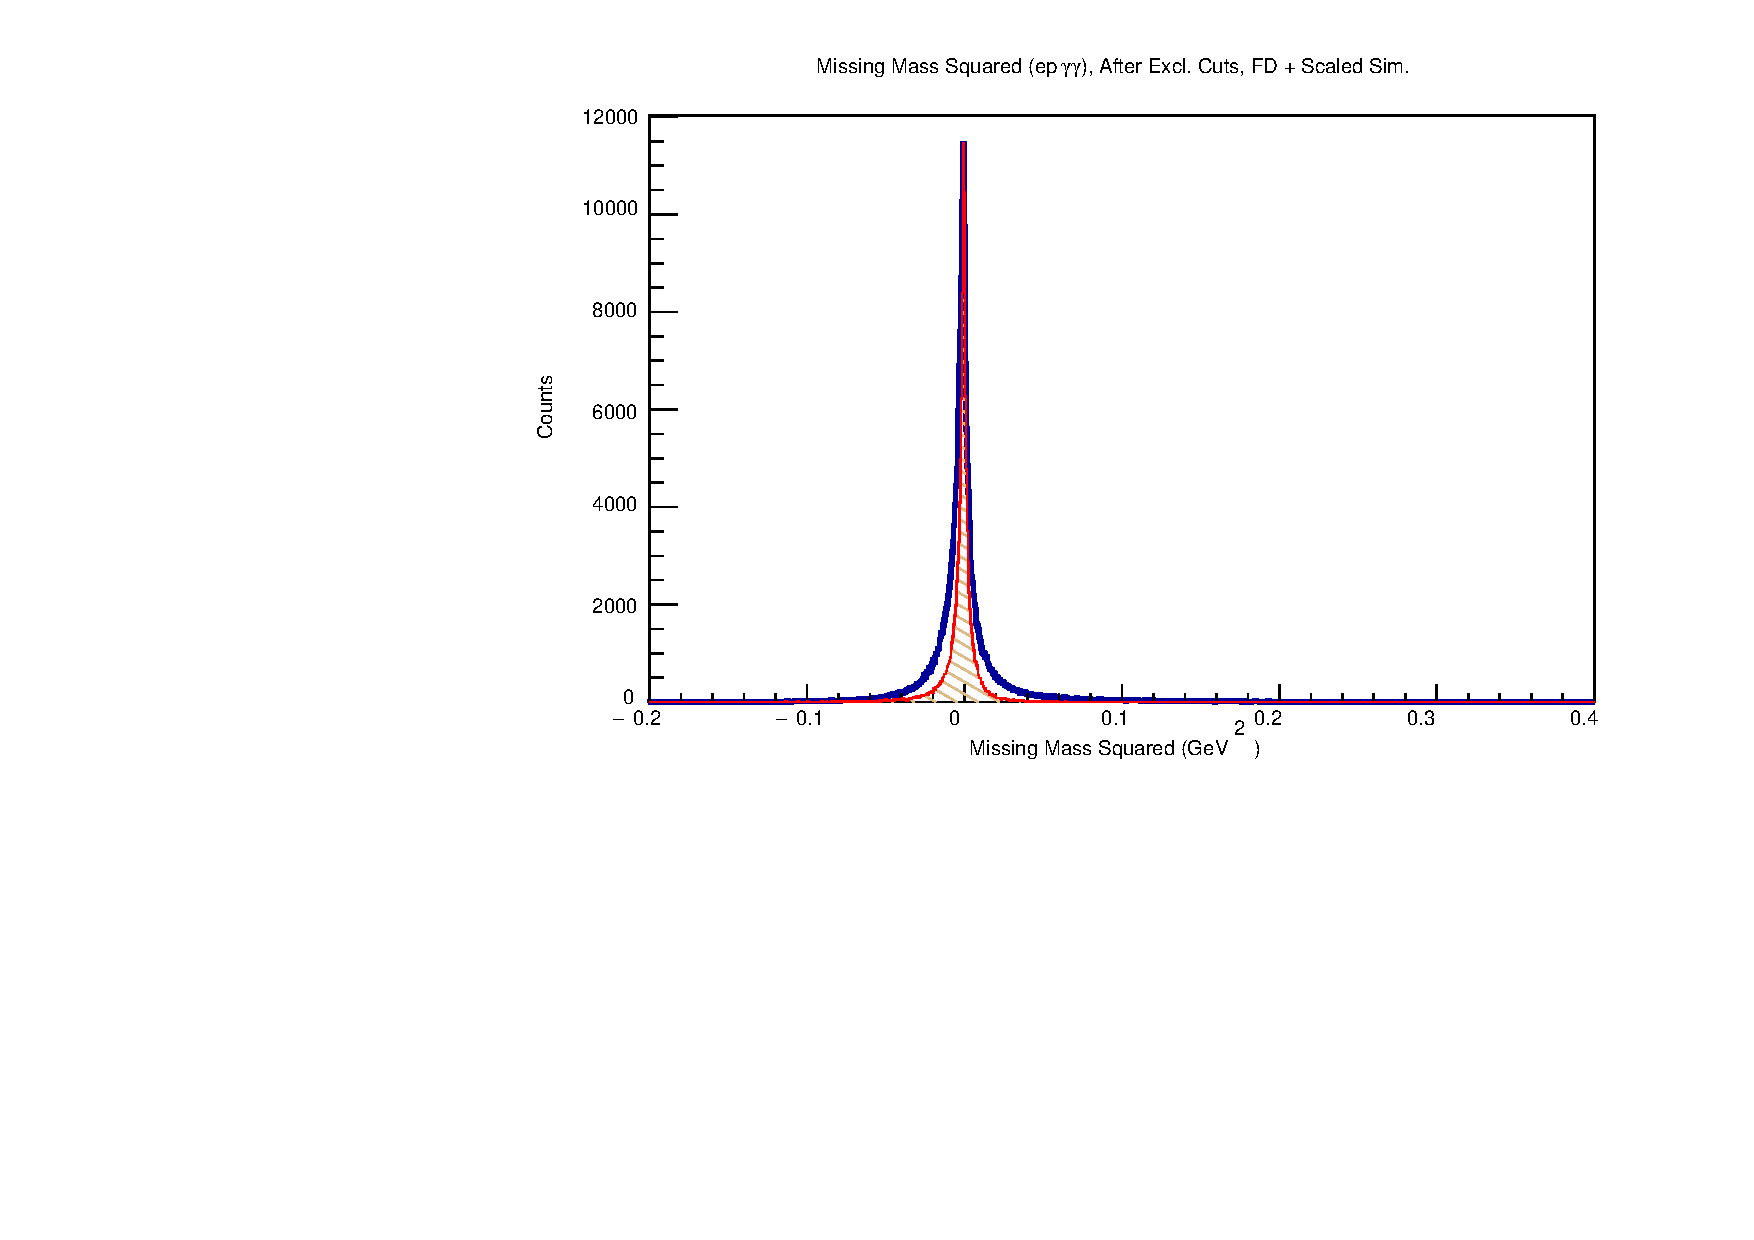
\includegraphics[width=1\textwidth]{figures/Simulation/exclusivity/hist_missing_mass_squared_epgg_excut_fd_Double.pdf}
            \end{subfigure}
            \caption[short]{Missing mass squared (epX) (top row and middle row (zoomed on middle row)) and missing mass squared (ep$\gamma \gamma$ distributions, before exclusivity cuts (left) and after (right) for data (blue) and simulation (red)}
        \label{fig:MM}
        \end{figure}

    \clearpage
    
    
    \section{Missing Energy}
    Finally, \ref{fig:ME} shows the missing energy distributions for the (epX) and (ep$\gamma \gamma$) systems. For exclusive $ep\pi^0$ events, $MM_{ep\gamma\gamma}$ = 0, and we do indeed see a peak centered around 0 for this distribution, with a strong agreement between data and simulation.

    \begin{figure}[!htb]
        \centering
        \begin{subfigure}{.5\textwidth}
            \centering
            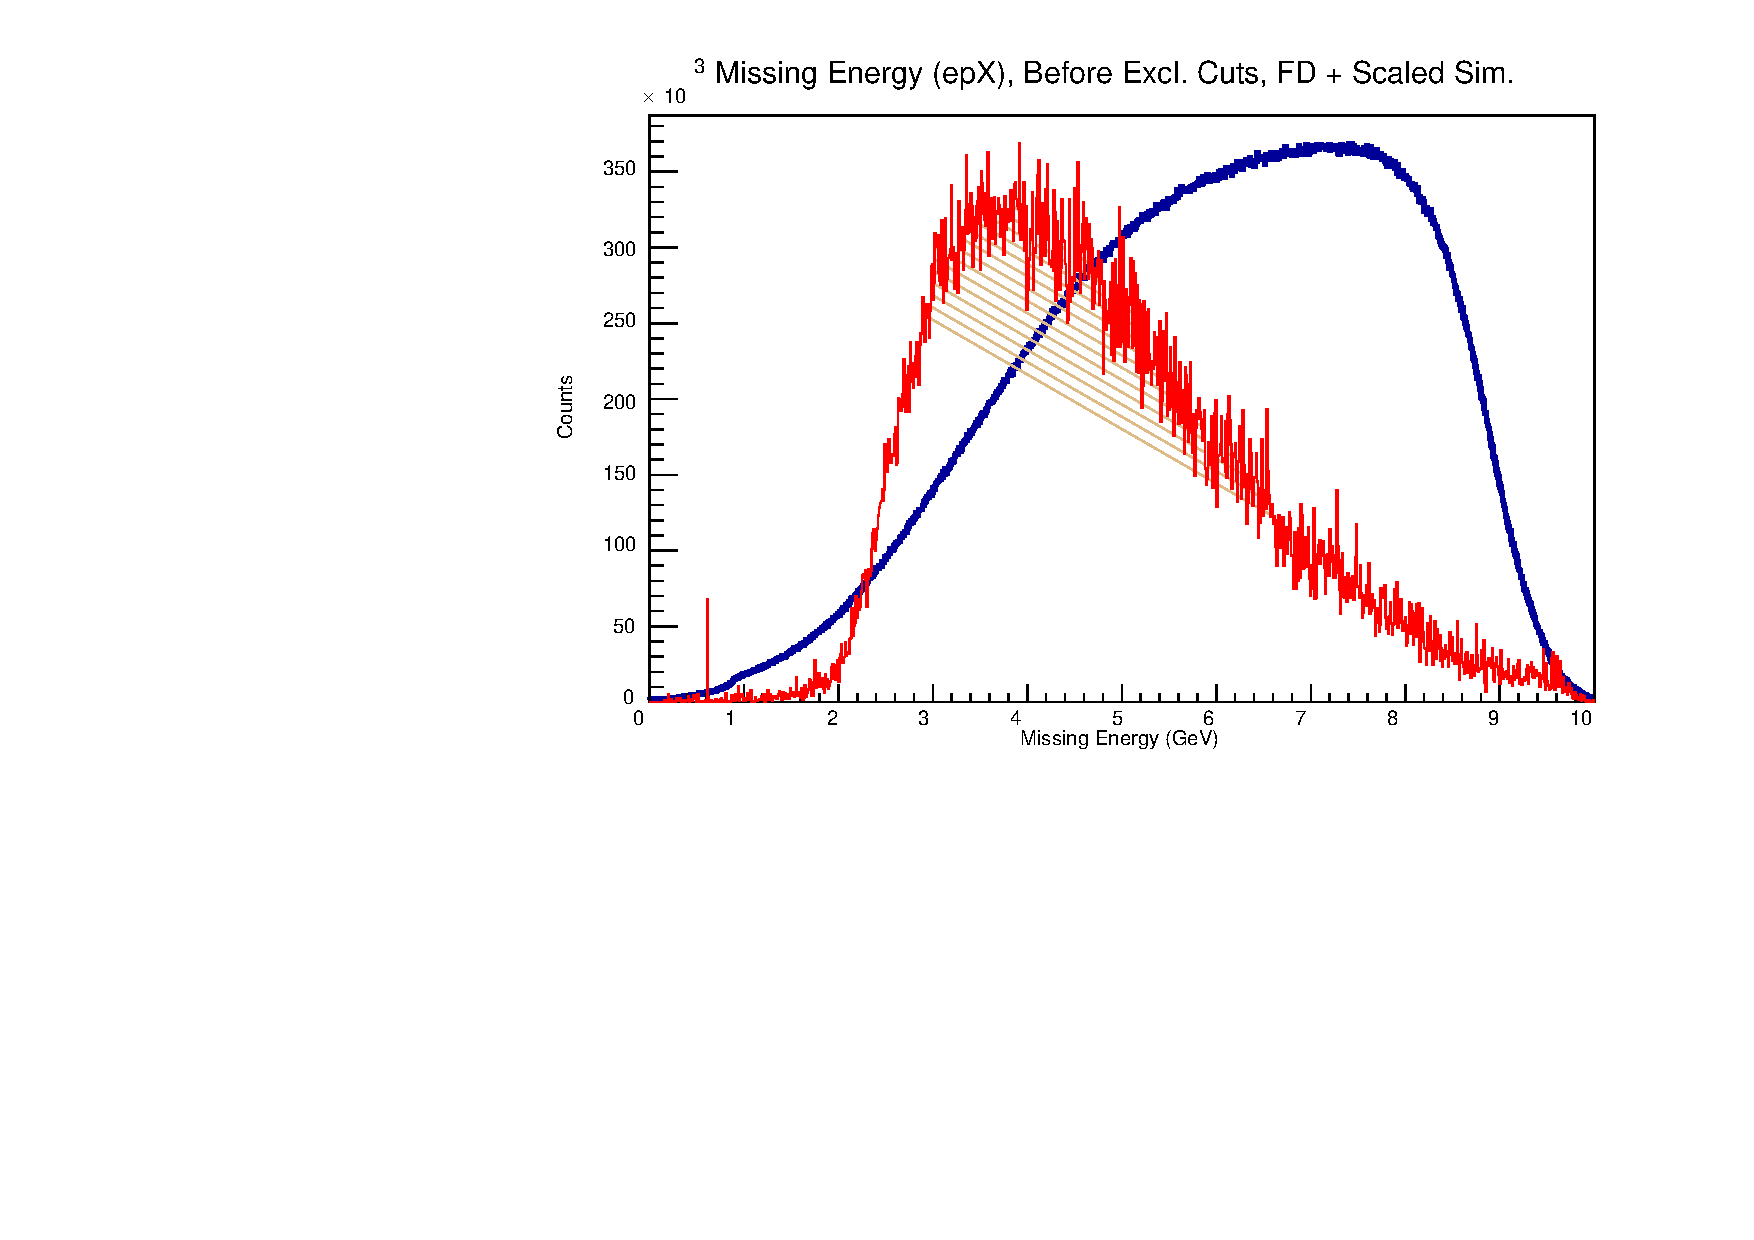
\includegraphics[width=1\textwidth]{figures/Simulation/exclusivity/hist_missing_energy_epx_prexcut_fd_Double.pdf}
        \end{subfigure}%
        \begin{subfigure}{.5\textwidth}
            \centering
            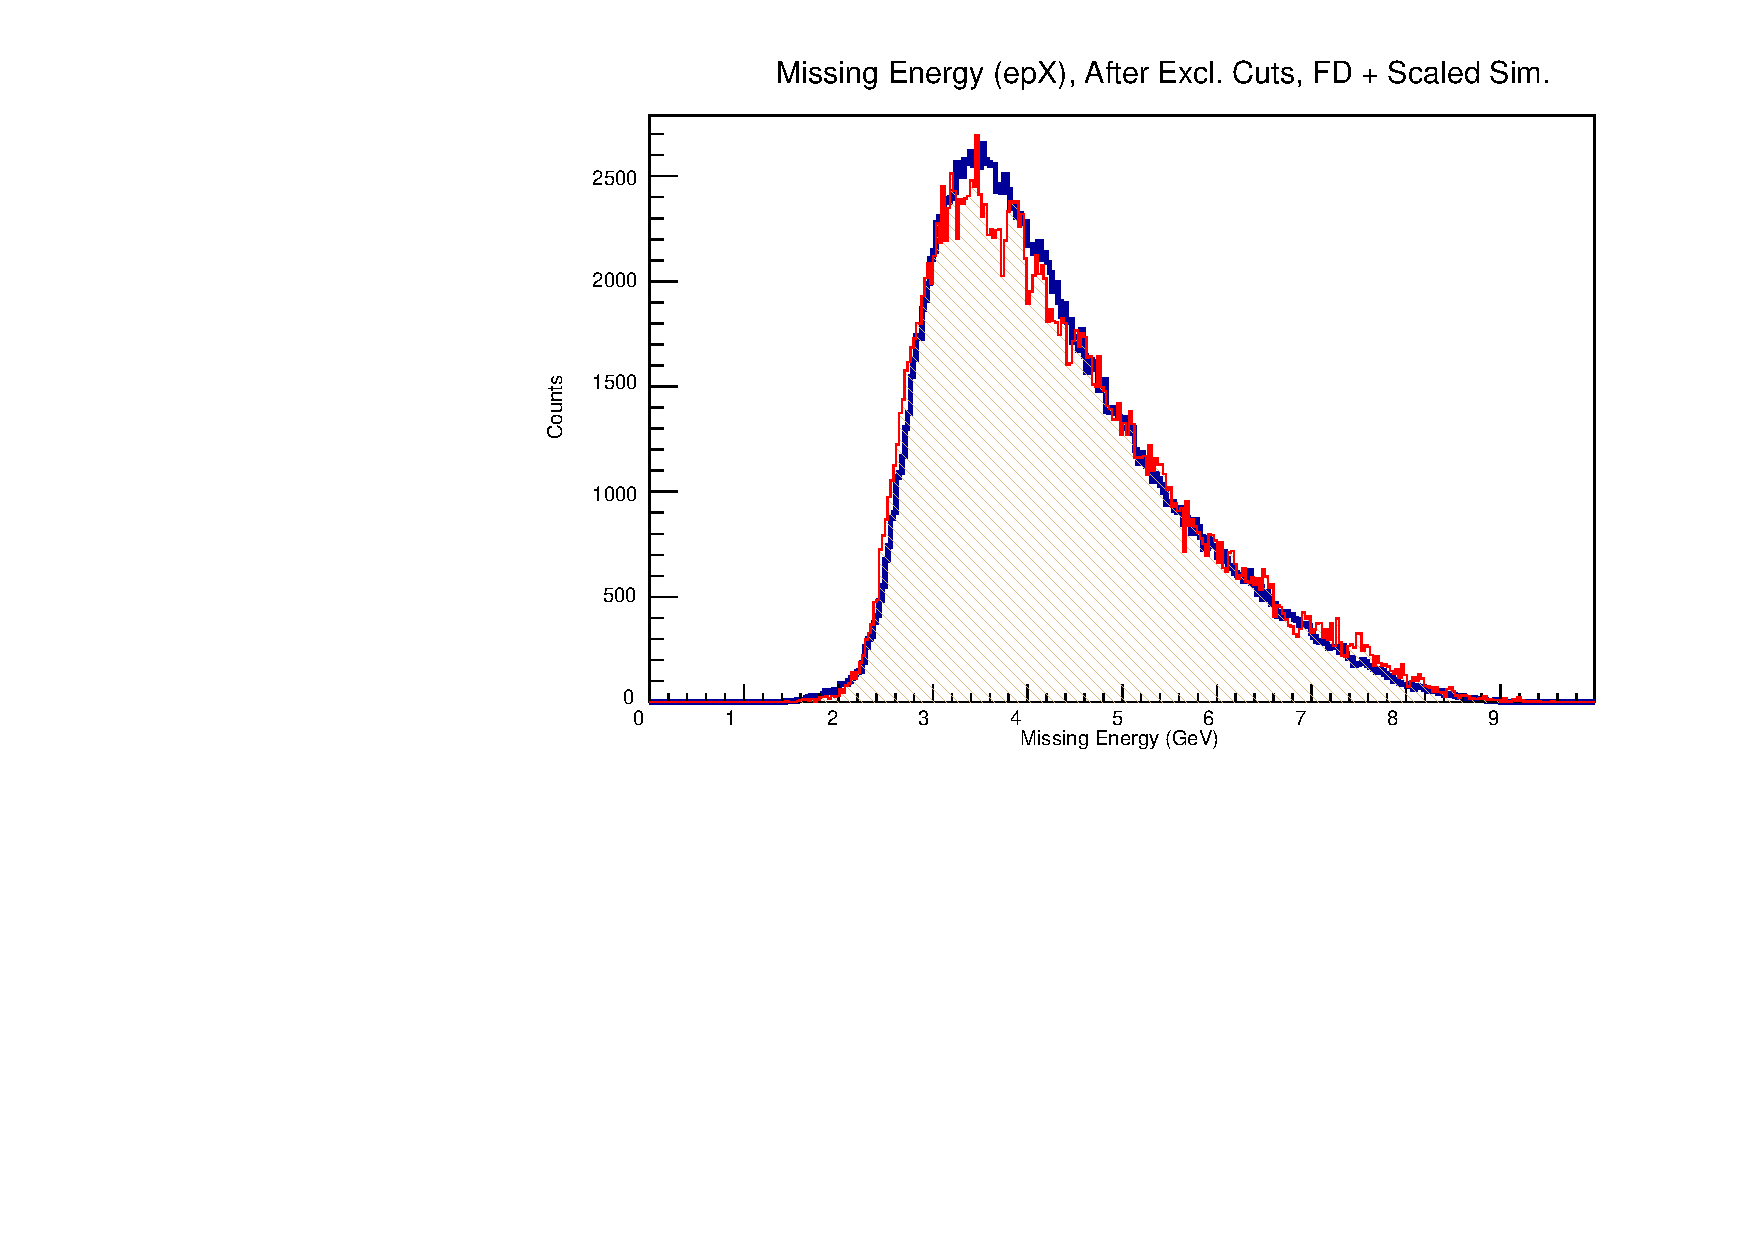
\includegraphics[width=1\textwidth]{figures/Simulation/exclusivity/hist_missing_energy_epx_excut_fd_Double.pdf}
        \end{subfigure}
        \begin{subfigure}{.5\textwidth}
            \centering
            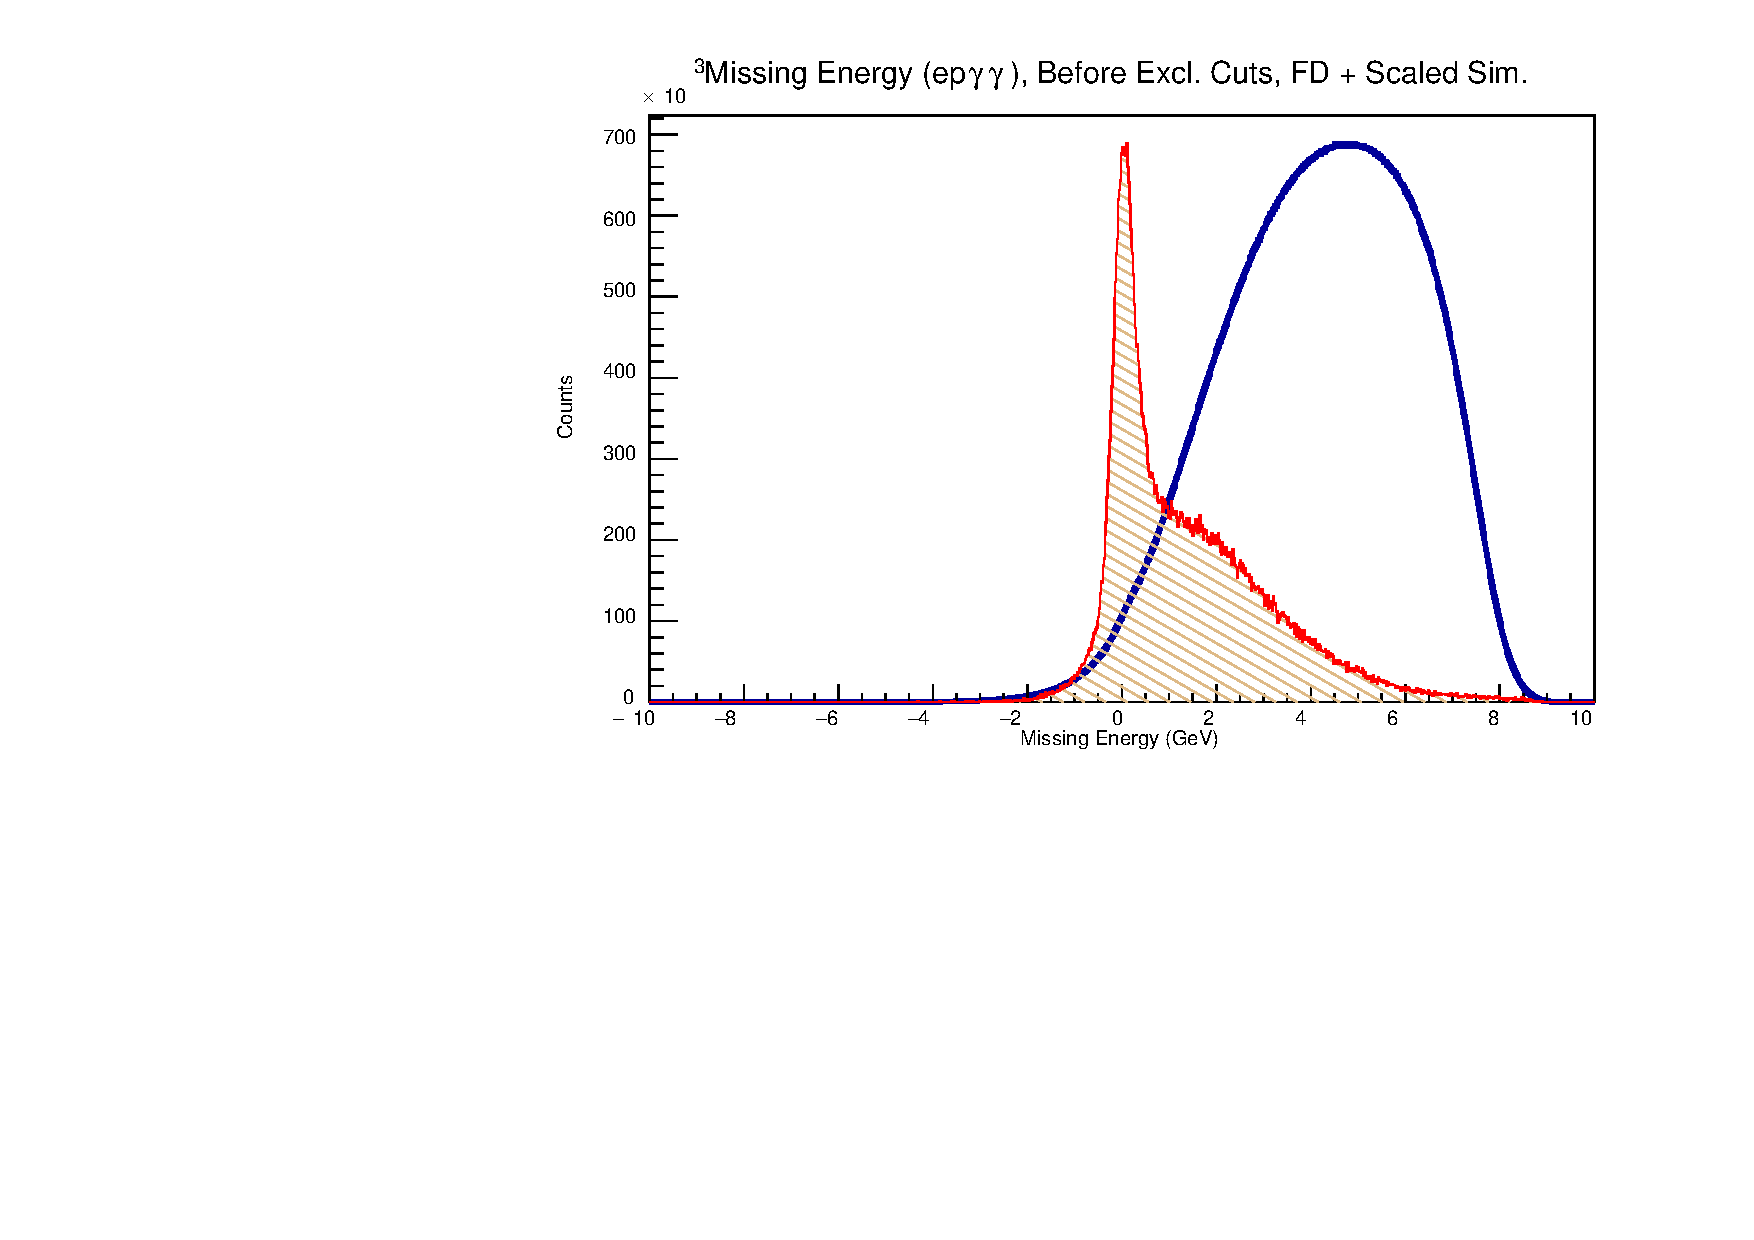
\includegraphics[width=1\textwidth]{figures/Simulation/exclusivity/hist_missing_energy_epgg_prexcut_fd_Double.pdf}
        \end{subfigure}%
        \begin{subfigure}{.5\textwidth}
            \centering
            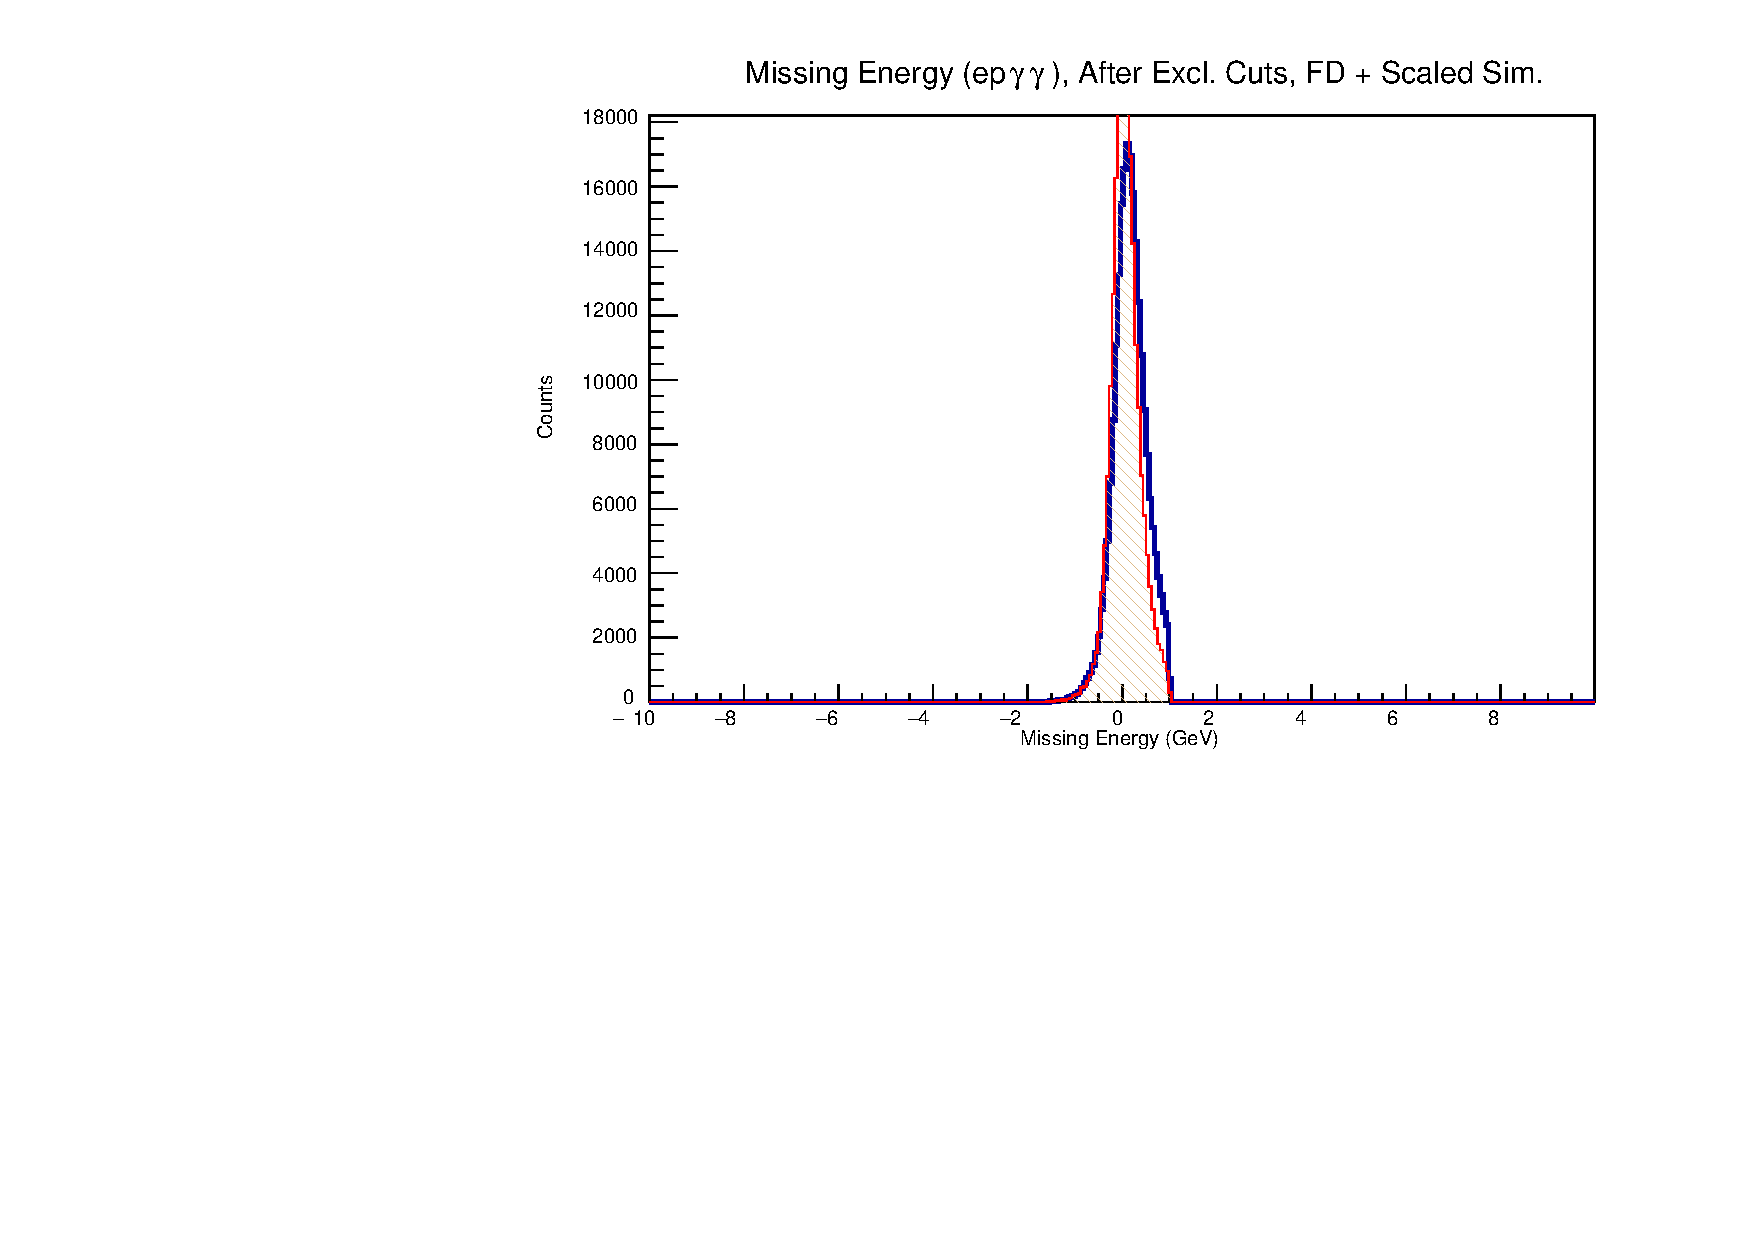
\includegraphics[width=1\textwidth]{figures/Simulation/exclusivity/hist_missing_energy_epgg_excut_fd_Double.pdf}
        \end{subfigure}
        \caption[short]{Missing energy (epx) (top) and missing energy (epgg) (bottom) distributions, before exclusivity cuts (left) and after (right) for data (blue) and simulation (red)}
    \label{fig:ME}
    \end{figure}
    
    
    \clearpage